% !TeX spellcheck = cs_CZ
%{\tikzset{external/prefix={tikz/FYZI/}}
% \tikzset{external/figure name/.add={ch01_}{}}
%---------------------------------------------------------------------------------------------------
% file fey1ch01_02_03.tex
%---------------------------------------------------------------------------------------------------
\definecolor{Gray}{gray}{0.9}
%===================== Kapitola: Základy fyziky ====================================================
\chapter{Základy fyziky}\label{fyz:IchapI}
\epigraph{\emph{Fyzika je jako sex, může přinést praktické výsledky, ale to není důvod, proč to 
  děláme.}}{Richard P. Feynmann}

\minitoc

  \begin{figure}[ht!]  % \ref{fyz:fig067}
    \centering
    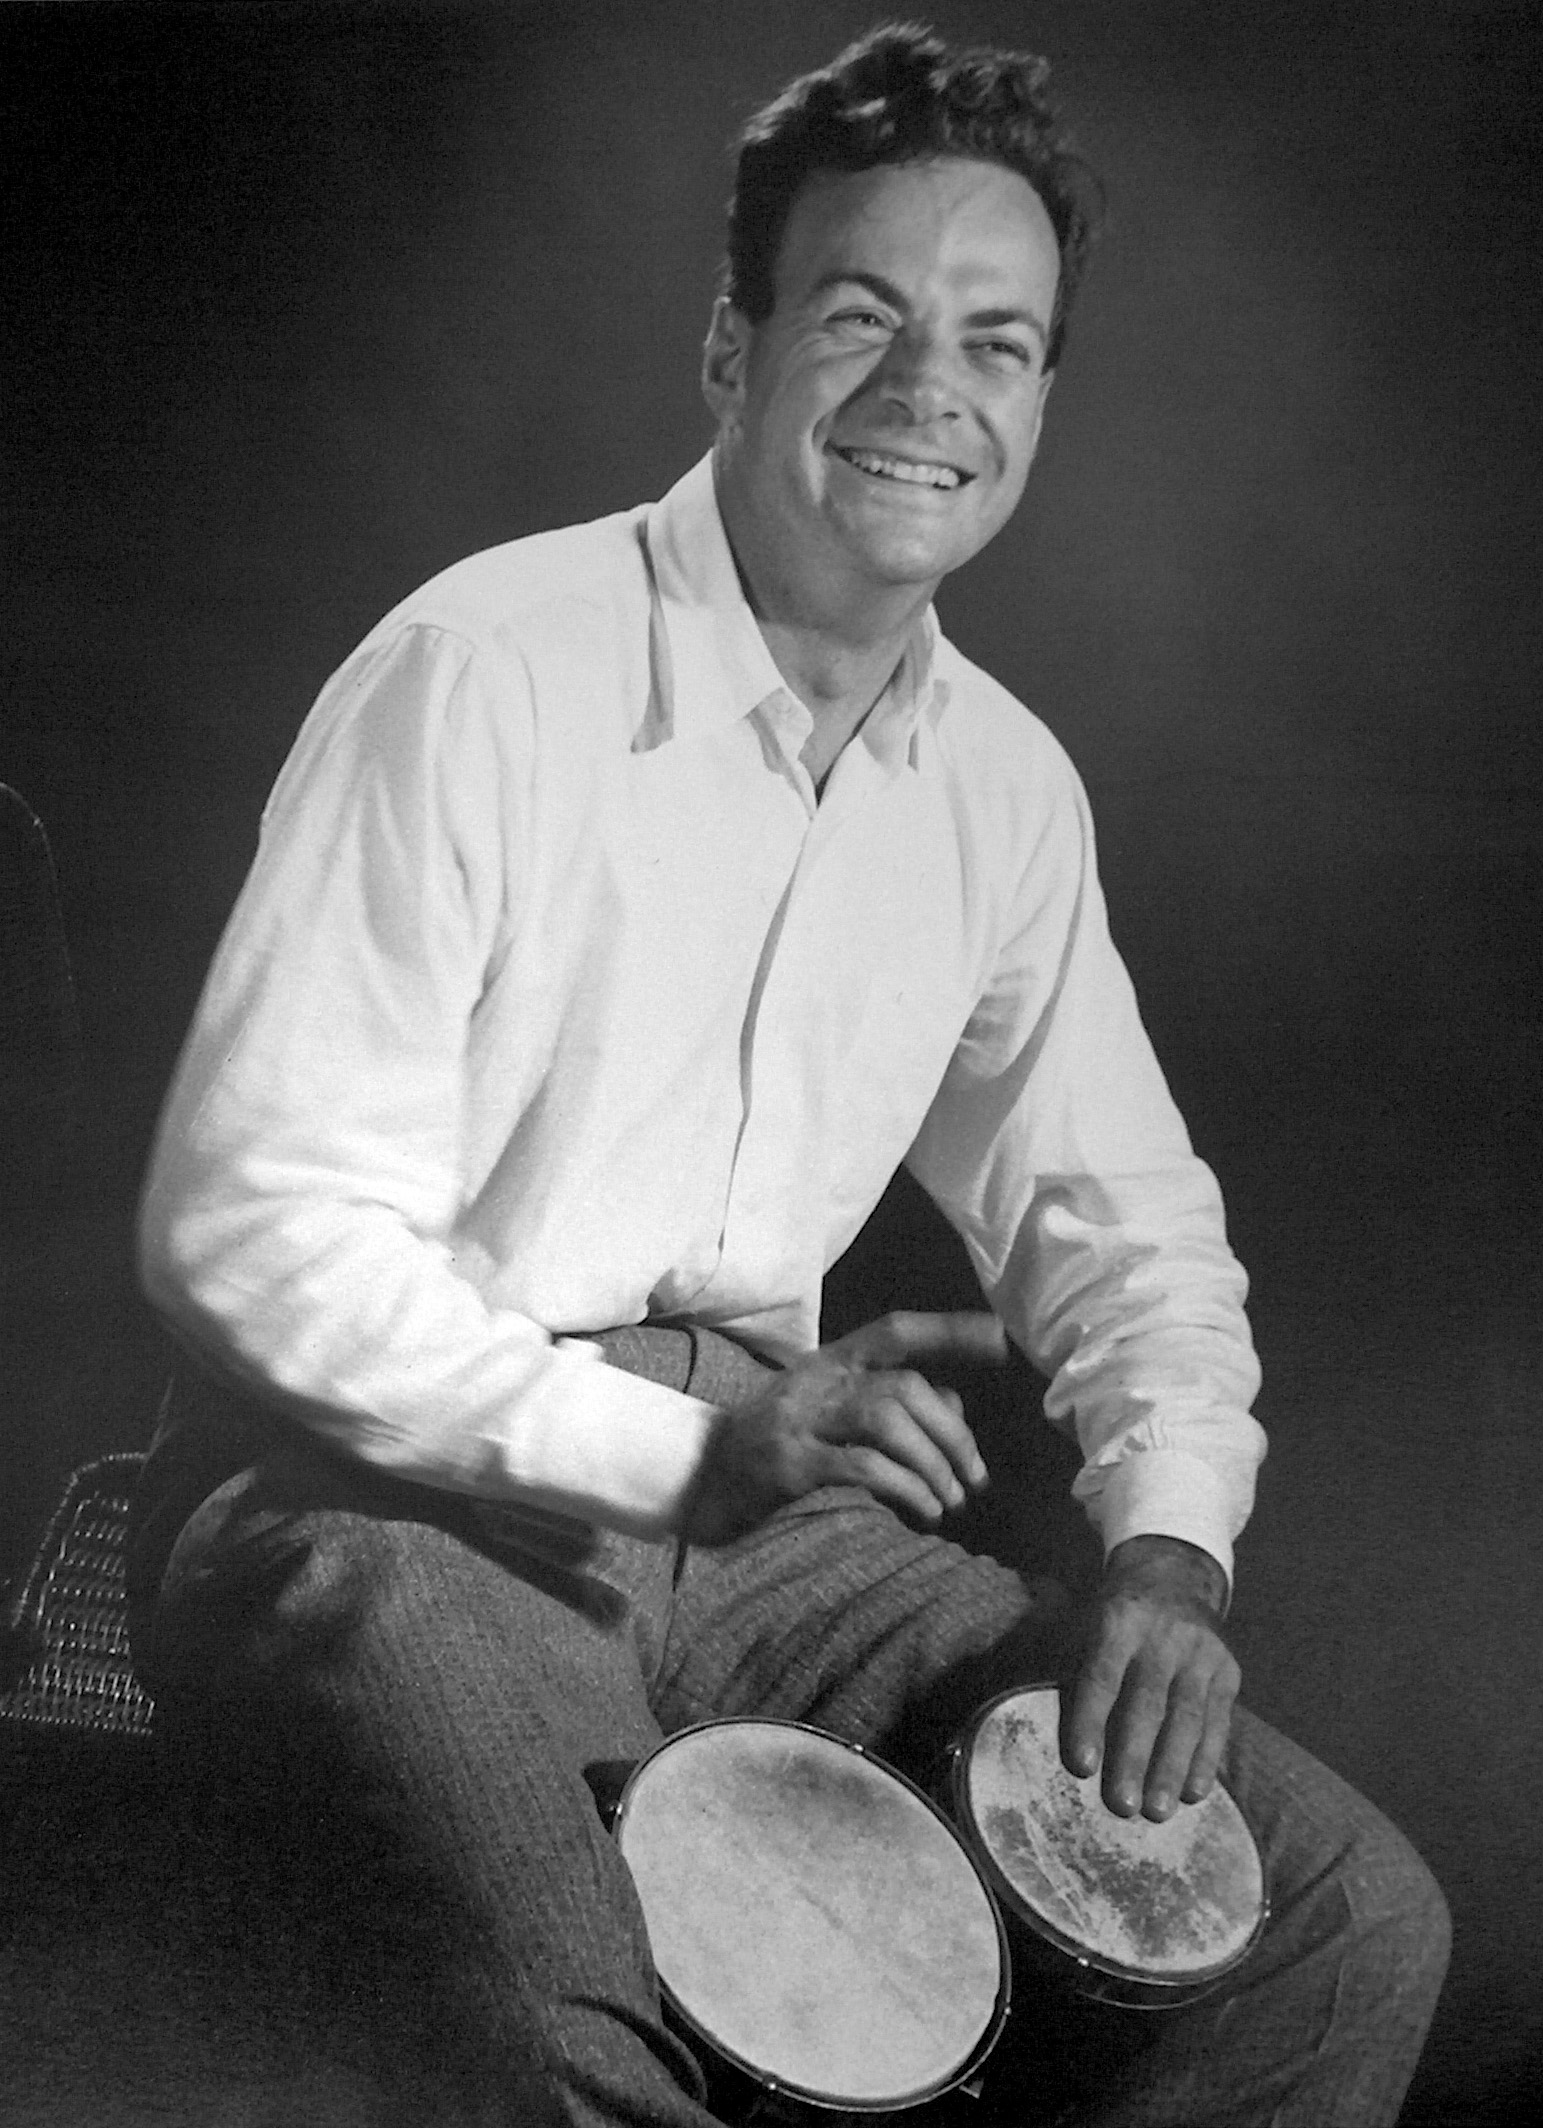
\includegraphics[width=0.6\linewidth]{fyz_fig067.jpg}
    \caption{\wikiFeynman \textasteriskcentered 11. května 1918 - \textdagger 15. února 1988, 
             americký fyzik, který patřil k největším fyzikům 20. století}
    \label{fyz:fig067}
  \end{figure} 

    Možná se zeptáte, zda není možné při vyučování fyziky na první straně uvést základní zákony a 
    potom ukázat, co z nich vyplývá v nejrůznějších situacích. Tak se postupuje v euklidovské 
    geometrii, kde se postulují axiomy, ze kterých se odvodí všechny možné závěry. (Protože se vám 
    nelíbí pětileté studium fyziky, chtěli byste seji naučit za pět minut?) Takovýmto způsobem však 
    nemůžeme postupovat ze dvou důvodů. Především, zatím neznáme všechny základní zákony - oblast 
    toho, co bychom ještě měli poznat, se nám stále zvětšuje. Dále, přesná formulace fyzikálních 
    zákonů zahrnuje mnoho neobvyklých myšlenek, jejichž vyjádření si vyžaduje vyšší matematiku. 
    Proto je nutná značná předběžná příprava jen k tomu, abychom rozuměli, co znamenají slova. Není 
    tedy možné postupovat tímto způsobem. \emph{Učit se můžeme pouze postupně, kousek po kousku}.

  \section{Jak studovat fyziku}\label{fyz:IchapIsecI}
    Každý kousek nebo část celku, který představuje příroda, je vždy jen přiblížením k úplné 
    pravdě; přesněji k úplné pravdě, pokud ji známe. Ve skutečnosti vše, co víme, je jen určitým 
    druhem aproximace, protože víme, ze ještě neznáme všechny zákony. Proto se věci musíme učit jen 
    proto, abychom se je znovu odnaučili, nebo, což je pravděpodobnější, abychom si naše znalosti o 
    nich opravovali.
    
    Princip vědy, téměř její definice, je následující: Prověrkou všech našich vědomostí je 
    experiment. Experiment je jediné kritérium vědecké „pravdy“. Jenže co je zdrojem našich 
    vědomostí? Odkud pocházejí zákony, které prověřujeme? Samotný experiment nám pomáhá odvozovat 
    zákony v tom smyslu, že nám poskytuje náznaky, pokyny. Navíc je však potřebná představivost, 
    aby z těchto náznaků mohla vzniknout velká zobecnění - abychom v nich odhadli nádherný, 
    jednoduchý, ale neobyčejný obraz a potom experimentem prověřili správnost našeho odhadu. Tento 
    proces představivosti je tak těžký, že si fyzici rozdělili práci - teoretičtí fyzici 
    představivostí, dedukcí a odhadem odvozují nové zákony, ale neexperimentují; experimentální 
    fyzici dělají pokusy a přitom také uplatňují představivost, dedukci a odhad.
    
    Řekli jsme, že přírodní zákony jsou přibližné: že nejdříve nacházíme „nesprávné“ a až potom 
    „správné“. Jak však může být experiment „nesprávný“? Především z velmi jednoduchého důvodu - 
    náš přístroj není v pořádku a my jsme to nezpozorovali. Takové chyby se však zjišťují lehce. 
    Odhlédneme-li od těchto drobností, jak může být výsledek experimentu nesprávný? Jen v důsledku 
    nepřesnosti. Například, hmotnost předmětu se zdá být neměnná; rotující káča má stejnou hmotnost 
    jako káča v klidu. Tak byl objeven „zákon“: hmotnost je konstantní, nezávislá na rychlosti. O 
    tomto „zákonu“ se zjistilo, že je nesprávný. Ukázalo se, že hmotnost roste s rychlostí, ale k 
    značnému růstu jsou potřebné rychlosti blízké rychlosti světla. Správný zákon zní: je-li 
    rychlost tělesa menší než \SI{100}{\km\per\second}, je hmotnost konstantní s přesností na jednu 
    milióntinu. V takové aproximativní podobě je tento zákon správný. Někdo by si mohl myslet, že 
    prakticky není rozdíl mezi starým a novým zákonem. To je i není pravda. Pro běžné rychlosti je 
    jistě možné zapomenout na to, o čem jsme mluvili a používat jednoduchý zákon konstantní 
    hmotnosti jako dobré přiblížení. Při velkých rychlostech se však dopustíme chyby, a to tím 
    větší, čím větší je rychlost
    
    Ostatně, nejzajímavější je to, že z filozofického hlediska je tento aproximativní zákon zcela 
    nesprávný. Náš celkový obraz o světě musíme změnit, i kdyby se hmotnost měnila jen nepatrně. 
    Toto je svérázný znak filozofie nebo myšlenek stojících v pozadí zákonů. Někdy i velmi malý 
    efekt vyžaduje hlubokou změnu našich názorů.
    
    Čemu tedy máme dát přednost? Máme podat správné, ale nezvyklé zákony s jejich cizím a obtížným 
    pojetím jako je například teorie relativity, čtyřrozměrný prostoročas a podobně? Nebo máme 
    nejdříve vysvětlit jednoduchý zákon „konstantní hmotností“, který je pouze přibližný, ale 
    nevyžaduje náročné představy? První způsob je více vzrušující, nádhernější a zábavnější, ale s 
    druhým se jednodušeji začíná a představuje první krok ke skutečnému porozumění správného 
    zákona. Tento problém se vždy znovu objevuje při vyučování fyziky. V různých etapách ho musíme 
    řešit různými způsoby, ale vždy je vhodné se zajímat, do jaké míry je přesné to, co teď víme, 
    jak to souvisí s dalším a jak se to může změnit, budeme-li vědět víc.
    
    Nyní přejděme k náčrtu nebo k všeobecné mapě našeho chápání současné vědy (zejména fyziky, ale 
    i jiných věd, které s ní souvisejí). Když se později soustředíme na konkrétní problém, budeme 
    mít představu o jeho pozadí, o tom, proč je zajímavý a jak zapadá do celkové struktury. Jaký je 
    tedy náš celkový obraz světa? \cite[s.~16]{Feynman01}
    
    \subsection{Látka se stává z atomů}
      Kdyby při nějaké katastrofě zanikly všechny vědecké poznatky a dalším generacím by měla 
      zůstat jen jediná věta, které tvrzení by při nejmenším počtu slov obsahovalo nejbohatší 
      informaci? Takovým kandidátem je \textbf{atomová hypotéza} - tj. že \emph{všechny věci se 
      skládají z atomů malých částic, jež jsou v neustálém pohybu,  a vzájemně se přitahují, když 
      jsou od sebe trochu vzdálené, ale odpuzují se, když jsou těsně u sebe.} V této jediné větě, 
      jak uvidíme, je obsaženo nesmírné množství informací o světě. Je k tomu třeba jen trochu 
      představivosti a uvažování.

      \begin{wrapfigure}[13]{r}{5cm}
        \centering
        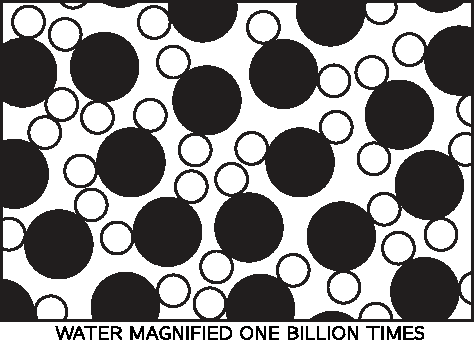
\includegraphics[width=0.9\linewidth]{fyz_fig007.pdf}
        \caption{Voda zvětšená miliardkrát \cite[s.~17]{Feynman01}}
        \label{fyz:fig_007}
      \end{wrapfigure} 
      Abychom ilustrovali sílu myšlenky o atomu, představme si kapku vody o rozměru \SI{0.5}{\cm}. 
      Podí\-váme-li se na ni zblízka, neuvidíme nic jiného, než vodu - klidnou, souvislou vodu. I 
      když kapku zvětšíme tím nejlepším optickým mikroskopem, přibližně dvoutisíckrát, a kapka bude 
      měřit deset metrů, tedy stejně jako velká místnost, i tehdy budeme stále vidět relativně 
      klidnou vodu. Jen tu a tam v ní budou plavat jakési malé fotbalové míče. Tyto velmi zajímavé 
      objekty jsou trepky. Tady se můžeme zastavit a zajímat se o trepky, o jejich třepotající se 
      řasičky, o jejich kroutící se těla a nepokračovat ve zvětšování. Nebo můžeme zvětšit trepky 
      tak, abychom viděli i do nich). Trepky jsou však předmětem biologie. Proto si jich teď 
      nebudeme všímat, ale zahledíme se ještě pozorněji na vodu při dalším dvoutisícinásobném 
      zvětšení. Teď měří kapka vody dvacet kilometrů a při pozorném sledování je vidět jakési 
      hemžení - cosi, co už nevypadá klidně, ale připomíná dav na fotbalové tribuně při pohledu z 
      velké vzdálenosti. Abychom zjistili, co je to za hemžení, zvětšíme kapku ještě 250krát a 
      potom uvidíme něco podobného jako na obr. \ref{fyz:fig_007}. Tento obrázek představuje vodu 
      při zvětšení miliardkrát, je však v několika směrech idealizovaný. Především částice jsou 
      zakreslené zjednodušeně - s ostrými okraji, což neodpovídá skutečnosti. Dále kvůli 
      jednoduchosti jsou částice zakreslené v dvojrozměrném uspořádání, ačkoli se ve skutečnosti 
      pohybují ve všech třech směrech. Všimněme si, že jsou tam dva druhy částic znázorněných 
      kroužky, které představují atomy kyslíku (černé) a vodíku (bílé) a že na každý atom kyslíku 
      se vážou dva atomy vodíku. Každá skupinka skládající se z atomu kyslíku a dvou atomů vodíku 
      se nazývá \textbf{molekulou}. Obrázek je zjednodušený i v tom, že skutečné částice v přírodě 
      se ustavičně kolébají a poskakují, obracejí se a točí jedna okolo druhé. Je třeba si to 
      představit spíše jako \emph{dynamický a nějako statický obrázek}. Další věcí, kterou není 
      možné vystihnout na obrázku, je skutečnost, že částice „drží pohromadě“ — přitahují se, jedna 
      za sebou táhne druhou atd. Je možné říci, že jsou jakoby „slepené dohromady“. Na druhé straně 
      se částice netlačí jedna přes druhou. Kdybyste se pokusili přitlačit dvě z nich příliš těsně 
      k sobě, odpudily by se.

      Atomy mají poloměr \SI{1e-10}{\m} až \SI{2e-10}{\m}. Jejich velikost si můžeme pamatovat i 
      jinak: zvětšíme-li jablko na velikost Země, budou atomy v jablku tak velké, jak bylo původně 
      jablko.

      Představme si teď tuto velkou kapku vody s jejími hemžícími se částicemi, jež přilnuly k sobě 
      a honí jedna druhou. Voda udržuje svůj objem; nerozpadne se na části díky vzájemné 
      přitažlivosti molekul. Je-li tato kapka na šikmé ploše, kde se může hýbat z místa na místo, 
      voda poteče. Nestane se však, že by jednoduše zmizela. Věci se nerozpadají na části právě 
      díky přitažlivosti molekul. \emph{Hemživý pohyb částic je to, co chápeme jako teplo}: 
      zvýšíme-li teplotu, zvětšíme pohyb. Zahříváme-li vodu, pohyb roste a roste i vzdálenost mezi 
      částicemi, až nastane okamžik, kdy přitažlivost mezi molekulami je už nestačí udržet 
      pohromadě. Částice přestanou být vzájemně svázané a rozlétají se od sebe. Zvyšováním teploty 
      tak získáváme \emph{vodní páru}.  
      
      \begin{wrapfigure}[12]{r}{5cm}
        \centering
        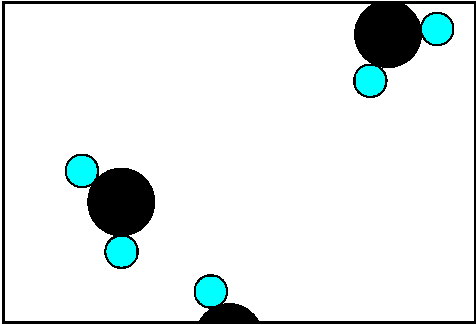
\includegraphics[width=0.9\linewidth]{fyz_fig008.pdf}
        \caption{Pára \cite[s.~18]{Feynman01}}
        \label{fyz:fig_008}
      \end{wrapfigure}
      Na obr. \ref{fyz:fig_008} vidíme páru. V jednom směru tento obrázek páry selhává: při našem 
      zvětšení za normálního atmosférického tlaku připadá jen velmi málo molekul na celý pokoj, 
      takže na tak malém obrázku určitě nebudou tři molekuly. Většina plošek této velikosti nebude 
      obsahovat žádnou molekulu - na našem obrázku jsou náhodou dvě a část z třetí molekuly 
      (abychom tam neměli prázdné místo). V případě páry vidíme podobu molekul jasněji než v 
      případě vody. Pro jednoduchost jsou molekuly zakresleny tak, že atomy vodíku svírají úhel 
      \SI{120}{\degree}. Ve skutečnosti má tento úhel hodnotu \ang[arc-separator = \,]{105;3;} a 
      vzdálenost mezi středem vodíku a středem kyslíku je \SI{9.57e-11}{\m}. Tuto molekulu tedy 
      velmi dobře známe.

      Všimněme si jedné vlastnosti vodní páry nebo jiných plynů. Molekuly budou tím, že se vzdálily 
      jedna od druhé, narážet na stěny. Představme si místnost s určitým počtem (tak kolem sta) 
      neustále poskakujících tenisových míčků. Když míčky narážejí na stěnu, odtlačují ji a stěnu 
      proto musíme upevnit. Plyn působí přerušovanou silou, kterou naše nedokonalé smysly (jejich 
      citlivost nevzrostla miliardkrát) vnímají jako \emph{stálý tlak}. Abychom plyn udrželi, 
      musíme na něj působit tlakem z opačné strany. Obr. \ref{fyz:fig_009} znázorňuje běžnou nádobu 
      na udržování plynu, kterou najdeme v každé učebnici: \textbf{válec s pístem}. Teď nám 
      nezáleží na tom, jaký je ve skutečností tvar molekul vody, a proto je kvůli jednoduchostí 
      znázorníme jako tenisové míčky nebo body. Jsou v neustálém pohybu a pohybují se na všechny 
      strany. Na spodek \emph{pístu} jich neustále naráží tolik, že na něj musíme působit určitou 
      silou dolů, aby ho molekuly nevytlačily z válce. Tuto \emph{sílu} nazýváme \textbf{tlakem} 
      (přesněji, \emph{tlak násobený plochou dává sílu}). Je jasné, že síla je úměrná ploše pístu, 
      protože zvětšíme-li plochu a přitom nezměníme počet molekul v kubickém centimetru, pak 
      vzroste počet srážek s pístem tolikrát, kolikrát se zvětšila jeho plocha.

      \begin{wrapfigure}[16]{r}{3cm}
        \centering
        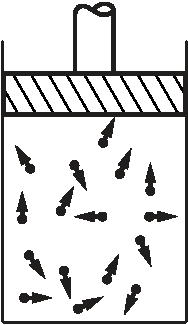
\includegraphics[width=0.9\linewidth]{fyz_fig009.pdf}
        \caption{Píst \cite[s.~18]{Feynman01}}
        \label{fyz:fig_009}
      \end{wrapfigure}
      Nyní \emph{zdvojnásobme} v této nádobě počet molekul, takže se zdvojnásobí jejich hustota, 
      ale ponechme jim stejnou rychlost, tj. \emph{stejnou teplotu}. Pak můžeme dost přesně říci, 
      že se zdvojnásobil počet srážek a jelikož je každá právě tak \uv{energická} jako dříve, tlak 
      je úměrný hustotě. Uvážíme-li skutečnou povahu meziatomových sil, můžeme očekávat mírný 
      pokles tlaku jako projev zvýšené přitažlivosti mezi atomy a mírný vzrůst související s 
      objemem, který zaujímají.Přesto však, pokud je hustota dostatečně nízká, tj. atomů není 
      příliš mnoho, můžeme s dostatečnou přesností říci, že \emph{tlak je úměrný hustotě}.
      
      Snadno pochopíme i něco jiného. \emph{Zvyšujeme-li teplotu} bez změny hustoty plynu, tj. když 
      zvětšujeme rychlost atomů, co se stane s tlakem? Atomy narážejí do pístu \emph{silněji}, 
      neboť se pohybují rychleji a navíc, narážejí častěji. Proto tlak vzrůstá. Vidíte, jak 
      jednoduché jsou myšlenky atomové teorie.
      
      Podívejme se na jinou situaci. Předpokládejme, že se píst \emph{pohybuje dovnitř}, takže 
      atomy jsou pomalu stlačovány do menšího prostoru. Co se stane, narazí-li atom do pohybujícího 
      se pístu? Je jasné, že při takové srážce \emph{získá rychlost}. Můžeme si to vyzkoušet na 
      ping-pongovém míčku: po úderu pálkou míček odletí od pálky rychleji, než k ní přiletěl. Ve 
      zvláštním případě, není-li atom v pohybu a píst na něj narazí, atom se začne určitě 
      pohybovat. Atomy jsou při návratu od pístu \uv{teplejší}, než byly před nárazem na píst. 
      Proto všechny atomy, které jsou v nádobě, získají na rychlosti. To znamená, že při pomalém 
      \emph{stlačení plynu jeho teplota vzrůstá}. Když plyn pomalu \emph{stlačujeme}, jeho teplota 
      \emph{vzrůstá} a když plyn pomalu \emph{rozpínáme}, jeho teplota \emph{klesá}.
      
      \begin{wrapfigure}[12]{r}{5cm}   % \ref{fyz:fig_010}
        \centering
        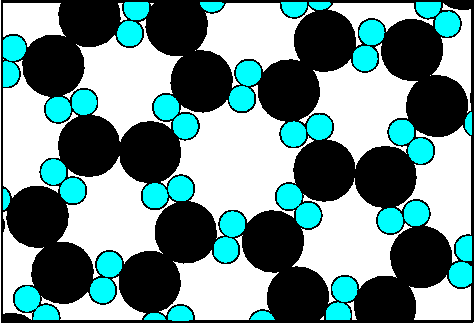
\includegraphics[width=0.9\linewidth]{fyz_fig010.pdf}
        \caption{Led \cite[s.~19]{Feynman01}}
        \label{fyz:fig_010}
      \end{wrapfigure}
      Vraťme se k naší kapce vody a podívejme se na ni z jiného pohledu. Snižme teplotu naší kapky. 
      Předpokládejme, že hemžení molekul vody postupně slábne. Víme, že mezi atomy působí 
      přitažlivé síly, které způsobí, že molekuly už nebudou moci tak snadno pohybovat. Obr. 
      \ref{fyz:fig_010} znázorňuje, co se stane při velmi nízkých teplotách: molekuly jsou vázány v 
      nové struktuře, vytváří se \textbf{led}. Takové schematické znázornění ledu není správné, 
      neboť je dvojrozměrné. Situaci však vystihuje kvalitativně. Je pozoruhodné, že každý atom má 
      v této látce určité místo. Rozmístíme-li atomy na jednom konci kapky podle určitého pravidla, 
      pak v důsledku pevné struktury meziatomových vazeb vznikne určité uspořádání atomů i na 
      druhém konci kapky, vzdáleném (v našem měřítku) několik kilometrů. Proto, držíme-li ledový 
      rampouch za jeden konec, jeho druhý konec bude při lámání klást odpor, chová se jinak než 
      voda, ve které je pravidelná struktura rozrušena intenzívním pohybem atomů v rozličných 
      směrech. Rozdíl mezi pevnými látkami a kapalinami spočívá v tom, že atomy pevné látky jsou 
      \emph{uspořádány} zvláštním způsobem. Toto uspořádání se nazývá \textbf{krystalická 
      struktura}. I tehdy, kdy jde o velmi vzdálené atomy, nepozorujeme nic náhodného v jejich 
      polohách. Poloha atomu na jednom konci krystalu je určena polohou atomu na druhém konci, i 
      když se mezi nimi nacházejí miliony jiných atomů. Obr. \ref{fyz:fig_010} znázorňuje vymyšlené 
      uspořádání ledu a ačkoli správně vystihuje mnohé vlastnosti ledu, neodpovídá skutečnému 
      uspořádání. Jedním ze správných rysů je existence části \emph{hexagonální symetrie}. Můžeme 
      se o tom přesvědčit: otočíme-li obrázek o \SI{120}{\degree}, dostaneme stejné seskupení. 
      Taková symetrie ledu je příčinou šestihranného tvaru sněhových vloček. Další informací, 
      kterou je možné vytušit z obrázku \ref{fyz:fig_010}, je \emph{zmenšování objemu ledu při 
      tání}. Znázorněná struktura ledu, stejně tak jako skutečná, obsahuje \emph{mnoho dutin}. Když 
      se struktura rozpadne, tyto dutiny mohou být \emph{zaplněny} molekulami. \emph{Většina 
      jednoduchých látek, s výjimkou vody a liteřiny, zvětšují při tání svůj objem, neboť atomy 
      jsou v pevných krystalech těsně seskupeny a při tání potřebují více prostoru na kmitání}. 
      Otevřené struktury se však při tání zhroutí - podobně jako led.
      
      I když má led pevnou krystalickou strukturu, jeho teplota se může měnit - v ledu je zásoba 
      tepla. Chceme-li, můžeme toto množství tepla změnit. Jaké je teplo, které se nachází v ledu? 
      Atomy ledu \emph{nejsou} v klidu, poskakují a kmitají. Ačkoli v krystalu existuje určité 
      uspořádání - struktura - všechny atomy kmitají, „na místě“. Zvyšujeme-li teplotu, budou 
      kmitat se stále větší amplitudou, až opustí svá místa. Tento jev nazýváme \textbf{táním}. 
      Snižujeme-li teplotu, kmity slábnou a při teplotě \emph{absolutní nuly} jsou 
      \emph{nejslabší}, ne však nulové. Toto nejmenší množství pohybu, který přísluší atomům, 
      nestačí na roztání látky - až na jednu výjimku: \emph{hélium}. V héliu se při ochlazování 
      také zpomaluje pohyb atomů na nejmenší možnou míru, ale i při teplotě absolutní nuly brání 
      tento pohyb zmrznutí hélia. Hélium nezmrzne, pokud nevytvoříme tak veliký tlak, abychom atomy 
      stlačili k sobě. Při velkém tlaku můžeme dosáhnout toho, že hélium ztuhne.
    
    \subsection{Atomové procesy}
      Dosud jsme si všímali stavby pevných látek, kapalin a plynů z atomového hlediska. Jenže 
      atomová hypotéza charakterizuje i procesy, a proto si všimněme některých procesů z atomového 
      hlediska. Nejdříve budeme hovořit o procesech, které se odehrávají na povrchu vody. Co se 
      vlastně děje na vodním povrchu? Úlohu si zkomplikujeme - bude tak blíže skutečnosti
      - předpokladem, že nad vodním povrchem se nachází vzduch. Obr. \ref{fyz:fig_011} takovou 
      situaci znázorňuje. Tak jako předtím vidíme molekuly vody, které tvoří kapalinu, ale vidíme i 
      povrch vody. Nad povrchem vidíme různé molekuly. Jsou tam především \emph{molekuly vody} v 
      podobě vodní páry, kterou je možné pozorovat vždy nad kapalnou vodou (pára a voda jsou v 
      rovnováze, o které pohovoříme později). Dále tam nalezneme jiné molekuly, dvojice atomů 
      kyslíku tvořící \emph{molekulu kyslíku} a dvojice atomů dusíku tvořící \emph{molekulu 
      dusíku}. Vzduch se skládá téměř výhradně z dusíku, kyslíku, vodní páry a menšího množství 
      oxidu uhličitého, argonu a jiných příměsí. Nad povrchem vody se nachází vzduch — plyn 
      obsahující jisté množství vodní páry. Nyní si všimněme, co se odehrává na obrázku. Molekuly 
      vody se neustále pohybují. Občas některá z molekul, nacházejících se v blízkosti povrchu, 
      naráží na jinou molekulu trochu silněji než obvykle a vyskočí nad povrch. Na obrázku takovýto 
      děj \emph{přímo} neuvidíme, neboť vše je na něm nehybné. Můžeme si však představit, že jedna 
      molekula za druhou v důsledku srážek opouštějí vodu - voda mizí, \emph{vypařuje} se. Když 
      nádobu \emph{přikryjeme}, objevíme po nějakém čase velké množství molekul vody mezi 
      molekulami vzduchu. Čas od času některá z těchto molekul vody vletí zpět do vody a zůstává v 
      ní. To, co jsme považovali za mrtvé a nezajímavé - přikrytý pohár vody, který snad dvacet let 
      stál na jednom místě - v sobě skrývá stále probíhající zajímavý \textbf{dynamický proces}. 
      Náš nedokonalý zrak nepozoruje žádnou změnu, ale při miliardovém zvětšení bychom viděli, jak 
      se vše mění: jedny molekuly opouštějí povrch a druhé se vracejí.
      
      \begin{wrapfigure}[14]{r}{5cm}   % \ref{fyz:fig_011}
        \centering
        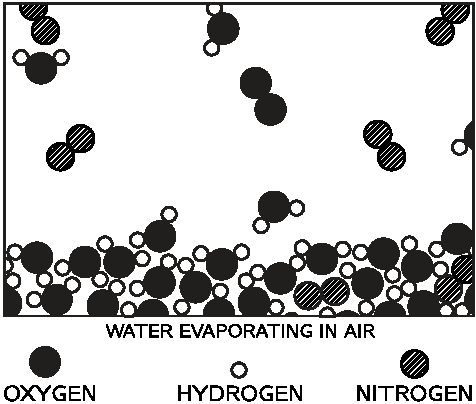
\includegraphics[width=0.9\linewidth]{fyz_fig011.pdf}
        \caption{Voda vypařující se do vzduchu \cite[s.~21]{Feynman01}.}
        \label{fyz:fig_011}
      \end{wrapfigure}
      Proč nepozorujeme tyto změny my? Protože do vody se vrací právě tolik molekul, kolik z ní 
      odešlo. Navenek se „nic neděje“. Když odkryjeme nádobu, odfoukneme vlhký vzduch pryč a 
      nahradíme ho suchým vzduchem, nezmění se počet z vody vylétajících molekul (neboť závisí 
      pouze na pohybu ve vodě), ale velmi se změní počet molekul do vody se vracejících, protože 
      nad vodou je mnohem méně molekul. Molekul, které opouštějí vodu, je víc než molekul, které se 
      do ní vracejí; voda se vypařuje. Chceme-li tedy, aby se voda vypařovala, zapneme ventilátor!
      
      \begin{wrapfigure}[15]{r}{5cm}   % \ref{fyz:fig_012}
        \centering
        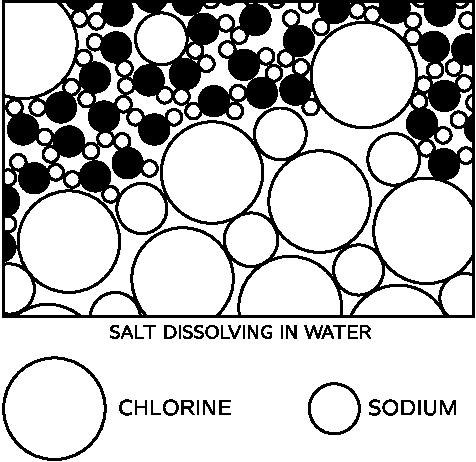
\includegraphics[width=0.9\linewidth]{fyz_fig012.pdf}
        \caption{Voda vypařující se do vzduchu \cite[s.~21]{Feynman01}.}
        \label{fyz:fig_012}
      \end{wrapfigure}
      Zůstává ještě otázka: Které molekuly opouštějí vodu? Molekula opustí vodu, když náhodně získá 
      malé množství dodatečné energie, kterou potřebuje na to, aby překonala přitažlivé působení 
      svých sousedů. Protože ty molekuly, které opouštějí vodu, mají větší než průměrnou energii, 
      budou se molekuly, které ve vodě zůstávají, v průměru pohybovat méně. Při vypařování se tedy 
      kapalina postupně \emph{ochlazuje}. Je samozřejmé, že když molekula páry sestoupí ze vzduchu 
      do vody, objeví se silné přitahování, když molekula dosahuje povrchu vody. Důsledkem toho je 
      zrychlení přicházející molekuly a s tím spojený vznik tepla. \emph{Můžeme tedy říci, že s 
      odchodem molekul odchází a s příchodem molekul přichází teplo.} Když jsou oba procesy 
      vyrovnány, voda svou teplotu nemění. Foukáme-li na vodu, aby odpařování převládalo nad 
      zkapalňováním, voda se ochlazuje. Proto, chcete-li ochladit polévku, foukejte na ni!
      
      Musíme si však uvědomit, že procesy, o kterých jsme hovořili, probíhají ve skutečnosti 
      složitěji. Při unikání vody do vzduchu čas od času některá z molekul kyslíku nebo dusíku 
      vnikne do vody a \uv{ztratí se} mezi jejími molekulami. Vzduch se tedy rozpouští ve vodě. 
      Molekuly kyslíku a dusíku pronikají do vody, která pak obsahuje vzduch. Když z nádoby náhle 
      odstraníme vzduch, budou molekuly vzduchu unikat z vody rychleji, než do ní vnikají, což 
      způsobí vystupování bublinek. Tato skutečnost je velmi nepříjemná pro potápěče.

      \begin{figure}[ht!]  % \ref{fyz:fig_013}
        \centering
        \begin{tabular}{c}
          \subfloat[ ]{\label{fyz:fig_013a}
            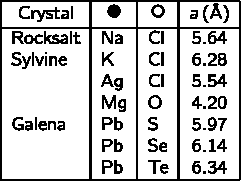
\includegraphics[width=0.2\textwidth]{fyz_fig013a.pdf}}
          \hspace{0.1\linewidth}                                                       \\
          \subfloat[ ]{\label{fyz:fig_013b}
            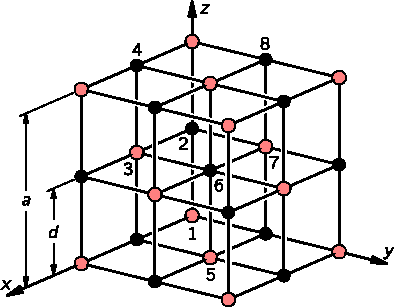
\includegraphics[width=0.3\textwidth]{fyz_fig013b.pdf}}
        \end{tabular}
        \caption{Vzdálenost nejbližších sousedů \(d = \dfrac{a}{2}\) \cite[s.~22]{Feynman01}}
        \label{fyz:fig_013}
      \end{figure}
      
      Nyní si všimněme dalšího procesu. Obr. \ref{fyz:fig_012} znázorňuje, jak se podle atomové 
      představy rozpouští pevná látka ve vodě. Co se stane, vložíme-li krystal soli do vody? Sůl je 
      pevná látka, krystal, organizované seskupení „atomů soli“. Na obr. \ref{fyz:fig_013} je 
      znázorněna trojrozměrná struktura kuchyňské soli, chloridu sodného. Máme-li být přesní, 
      musíme říct, že krystal není tvořen atomy, ale ionty. Iont je atom, který má několik 
      elektronů navíc, nebo několik elektronů ztratil. V krystalu soli nalézáme \emph{ionty chlóru} 
      (atomy chlóru s přebytečným elektronem) a \emph{ionty sodíku} (atomy sodíku zbavené jednoho 
      elektronu). Ionty jsou v krystalu vzájemně vázány elektrickou přitažlivostí, ale ve vodě se 
      některé z nich pod vlivem přitažlivosti záporného kyslíku a kladného vodíku začnou uvolňovat. 
      Na obrázku \ref{fyz:fig_012} vidíme uvolňující se iont chlóru a jiné atomy plavající ve vodě 
      ve formě iontů. Tento obrázek je pečlivě zakreslený. Všimněme si například, že vodíkové konce 
      molekul vody obvykle obklopují iont chlóru a u iontu sodíku zpravidla nalézáme kyslíkový 
      konec, neboť sodík je kladný a kyslíkový konec molekuly vody je záporný a tyto se elektricky 
      přitahují. Můžeme podle tohoto obrázku říci, jestli se sůl \emph{rozpouští} ve vodě, nebo 
      \emph{krystalizuje} z vody? Samozřejmě, že \emph{nemůžeme}, neboť zatím co jedny atomy 
      opouštějí krystal, jiné se k němu připojují. Takovýto proces je - podobně jako vypařování - 
      \emph{dynamický} všechno závisí na tom, je-li ve vodě více nebo méně soli, než je třeba k 
      rovnováze. Rovnováhou rozumíme takovou situaci, kdy počet atomů opouštějících krystal je 
      roven počtu atomů do krystalu se vracejících. Když sůl ve vodě téměř není, vstupuje do vody 
      více atomů, než vystupuje a sůl se rozpouští. Když je, naopak, „atomů soli“ příliš mnoho, do 
      krystalu se vrací více atomů, než ho opouští a sůl krystalizuje.
      
      Zmínili jsme se o tom, že představa \emph{molekuly} látky je pouze přibližná a je 
      opodstatněná jen pro určitou třídu látek. Je jasné, že v případě vody jsou její tři atomy 
      skutečně svázané, ale v případě pevného chloridu sodného už to tak jasné není. V takovém 
      případě jde o uspořádání sodíkových a chlorových iontů do krychlové mřížky a neexistuje 
      přirozený způsob jejich uspořádání do „molekul soli“.
      
      Vraťme se ještě k naší diskuzi o \emph{rozpouštění a srážení}. Zvýšíme-li teplotu roztoku 
      soli, vzroste počet atomů, které sůl opouštějí a vzroste i počet atomů, které se do soli 
      vracejí. Ukazuje se, že obecně je velmi těžké předpovědět, jak se ten proces realizuje, 
      proběhne-li rozpouštění rychleji nebo pomaleji. S rostoucí teplotou se většina látek 
      rozpouští lépe, ale některé látky se rozpouštějí hůře.
      
    \subsection{Chemické reakce}
      Ve všech procesech, o nichž jsem dosud hovořili, neměnily atomy a ionty své partnery. Za 
      určitých okolností však může dojít ke změně atomových kombinací, vytvoří se nové molekuly. 
      Taková situace je znázorněna na obr. \ref{fyz:fig_014}.
      
      \begin{wrapfigure}[12]{r}{5.1cm}   % \ref{fyz:fig_014}
        \centering
        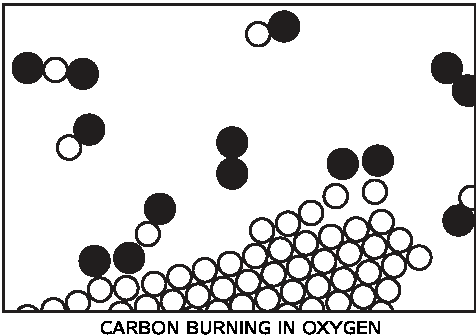
\includegraphics[width=0.9\linewidth]{fyz_fig014.pdf}
        \caption{Uhlík hořící v kyslíku \cite[s.~23]{Feynman01}}
        \label{fyz:fig_014}
      \end{wrapfigure}
      Proces, ve kterém dochází k přeskupení atomových partnerů, nazýváme \textbf{chemickou 
      reakcí}. Ostatní dosud uvažované procesy nazýváme \textbf{fyzikálními procesy}. Mezi 
      uvedenými dvěma druhy, procesů však neexistuje ostrá hranice. Příroda se nestará o naše 
      názvosloví a pokračuje i nadále ve svém díle. Uvedený obrázek má znázornit hoření uhlíku v 
      kyslíku. Kyslík se vyznačuje tím, že jeho dva atomy jsou velmi pevně svázány. (Proč nejsou 
      svázány \emph{tři} nebo dokonce \emph{čtyři} atomy? Toto je jedna ze zvláštností atomových 
      procesů. Atomy jsou velmi svérázné: upřednostňují určité partnery, určité směry apod. Úlohou 
      fyziky je analyzovat, proč chtějí právě to, co chtějí. V každém případě dva atomy kyslíku, 
      nasycené a šťastné, tvoří molekulu.)
      
      \begin{wrapfigure}[12]{r}{5.0cm}   % \ref{fyz:fig_015}
        \centering
        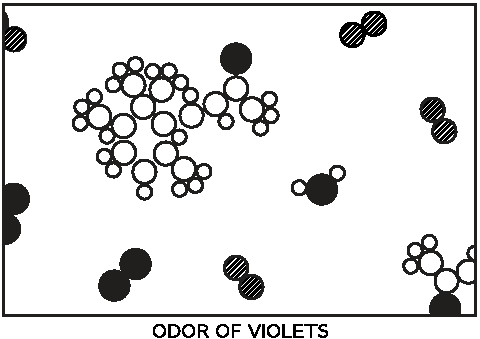
\includegraphics[width=0.9\linewidth]{fyz_fig015.pdf}
        \caption{Vůně fialek \cite[s.~24]{Feynman01}}
        \label{fyz:fig_015}
      \end{wrapfigure}
      Předpokládejme, že atomy uhlíku vytvářejí pevný krystal - grafit nebo diamant (diamant může 
      shořet ve vzduchu). Uvažujme situaci, kdy se molekula kyslíku dostane k uhlíku, Každý její 
      atom zachytí atom uhlíku a odletí v novém seskupení - „uhlík-kyslík“. Toto seskupení 
      představuje molekulu plynu nazývaného \emph{oxid uhelnatý}. Jeho chemické označení je 
      \ce{CO}. Je to velmi jednoduché: písmena „CO“ jsou vlastně obrazem jeho molekuly. Jenže 
      uhlík váže kyslík o mnoho silněji než kyslík váže kyslík nebo uhlík váže uhlík. Proto v tomto 
      procesu může kyslík přicházet s malou energií, ale kyslík a uhlík se spojí velmi „energicky“ 
      a uvolněnou energii pohltí okolní atomy. Tak se vytváří velké množství pohybové, kinetické 
      energie. Myslíme tím samozřejmě \textbf{hoření}; spojením uhlíku a kyslíku získáváme 
      \emph{teplo}. Teplo se obvykle projevuje formou pohybu molekul horkého plynu, ale za určitých 
      okolností ho může být tak mnoho, že způsobuje světlo. Tak vzniká \textbf{plamen}.
      
      Kromě toho, \emph{oxid uhelnatý} není zcela uspokojen. Je možné, aby k sobě připoutal další 
      atom kyslíku a tak dostaneme mnohem složitější reakci, ve které se kyslík spojuje s uhlíkem a 
      současně dochází ke srážce s molekulou oxidu uhelnatého. Kyslíkový atom se připojí k \ce{CO} 
      a v konečném důsledku vytvoří molekulu složenou z jednoho uhlíku a dvou kyslíků. Tato 
      molekula má označení \ce{CO2} a nazývá se \emph{oxid uhličitý}. Spalujeme-li uhlík ve velmi 
      malém množství kyslíku a reakce probíhá velmi rychle (např. v motoru automobilu, kde je 
      výbuch tak rychlý, že se nestačí vytvořit oxid uhličitý), vzniká velké množství oxidu 
      uhelnatého. V mnoha takových přeskupeních atomů se uvolňuje velké množství energie, vznikají 
      výbuchy, plamen apod., podle druhu reakce. Chemici studovali takové seskupení atomů a 
      zjistili, že každá látka představuje určitý druh \emph{uspořádání atomů}.

      K objasnění této myšlenky si zvolme jiný příklad. Ocitneme-li se na louce rozkvetlé fialkami, 
      víme, co je to za „vůni“. Je to určitý druh molekul nebo seskupení atomů, které se dostalo do 
      našeho nosu. Jak se nám to stalo? To je dost jednoduché! Jestliže vůně je jistý druh molekul, 
      tím nejrozmanitějším způsobem poletujících a srážejících se ve vzduchu, pak se může náhodou 
      dostat i do nosu. Tyto molekuly se určitě nesnažily dostat právě do našeho nosu. Jsou jen 
      bezmocnou částí strkajícího se zástupu molekul, jehož kousek se na svém bezcílném putování 
      dostal do našeho nosu.      
      
      Chemici mohou i takové zvláštní molekuly, jako je vůně fialek, podrobit analýze a říci nám 
      \emph{přesné uspořádání} jejich atomů v prostoru. Víme, že molekula oxidu uhličitého je 
      \emph{přímá a symetrická}: \ce{O\bond{-}C\bond{-}O} (lze to snadno zjistit i fyzikálními 
      metodami). I pro mnohem složitější seskupení atomů, jako jsou ty, se kterými pracuje chemie, 
      můžeme zdlouhavým, pozoruhodným procesem, připomínajícím práci detektiva, zjistit tvar 
      seskupení. Obr. \ref{fyz:fig_015} znázorňuje vzduch v blízkosti fialky: ve vzduchu opět 
      nalézáme dusík, kyslík a vodní páru. (Odkud se vzala vodní pára? Fialka je vlhká, protože 
      všechny rostliny odpařují vodu.) Vidíme však i \uv{monstrum} složené z uhlíkových, vodíkových 
      a kyslíkových atomů, které vytvořily zcela určité, zvláštní seskupení. Je to mnohem 
      složitější seskupení než v případě oxidu uhličitého. Naneštěstí do obrázku nemůžeme zakreslit 
      všechno, co o něm po chemické stránce víme, neboť seskupení všech atomů je trojrozměrné, 
      zatímco náš obrázek je pouze dvojrozměrný. Šest uhlíků vytváří ne plochý, ale \uv{zvrásněný} 
      prstenec. Všechny úhly a vzdálenosti známe. Chemický vzorec je jen obrázkem takové molekuly. 
      Když chemik napíše vzorec na tabuli, snaží se \uv{nakreslit} dvojrozměrný obraz molekuly. 
      Například, vidíme \uv{prstenec} šesti uhlíků a na jednom konci visící \uv{řetěz} uhlíků, na 
      něm kyslík druhý od konce, tři vodíky vázané na tento uhlík, dva uhlíky a tři vodíky vázané 
      nahoře atd.

      \begin{wrapfigure}[11]{r}{5cm}   % \ref{fyz:fig_016}
        \centering
        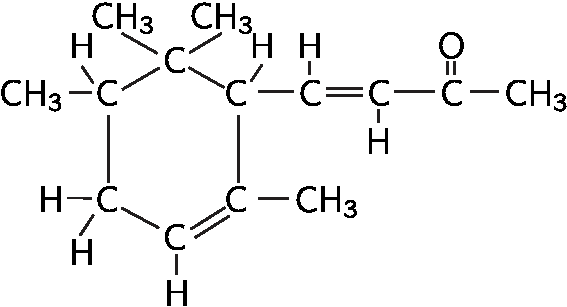
\includegraphics[width=0.9\linewidth]{fyz_fig016.pdf}
        \caption{Strukturní vzorec vůně fialky (\(\alpha\)-iron) \cite[s.~24]{Feynman01}}
        \label{fyz:fig_016}
      \end{wrapfigure}
      Jak chemik zjistí, o jaké uspořádání jde? Smíchá obsah dvou lahviček a když se směs zbarví 
      červeně, ví, že látka obsahuje jeden vodík a dva uhlíky vázané na určité místo molekuly. 
      Zbarví-li se směs modře, je to úplně jinak. To je organická chemie - jeden z 
      nejfantastičtějších kousků detektivní práce. Aby objevil uspořádání atomů v neobyčejně 
      komplikovaných útvarech, chemik sleduje, co se děje při smíchání dvou rozdílných látek. Fyzik 
      by nikdy zcela neuvěřil, že chemik ví, o čem mluví při popisu uspořádání atomů. Jenže asi 
      před dvaceti lety se objevila fyzikální metoda umožňující v některých případech pozorovat 
      molekuly (ne tak složité, jako je molekula vůně fialky, ale takové, které obsahují části této 
      molekuly). Touto metodou je možné lokalizovat každý atom, a to ne sledováním zbarvení směsi, 
      ale měřením skutečné polohy atomů. A světe, div se! Ukázalo se, že chemici měli téměř vždy 
      pravdu. Zjistilo se, že vůně fialky obsahuje tři málo se lišící molekuly, jejichž rozdílnost 
      spočívá pouze v jiném uspořádání vodíkových atomů. 
      
      Jedním z problémů chemie je tvorba chemického názvosloví. Každé molekule musíme najít jméno! 
      Toto jméno musí ukazovat nejen její tvar, ale musí vyjadřovat i to, že tu je kyslíkový atom, 
      tam vodíkový - musí říkat, kde přesně ten který atom je. Takto pochopíme, že chemické názvy 
      musí být složité, aby byly-úplné. Název fialkové vůně má v podobě prozrazující strukturu 
      následující znění: 4-(2,2,3,6 tetrametyl-5-cyklohexa\-nyl)-3-buten-2-on. Teď chápeme obtíže, 
      se kterými chemici zápolí a rovněž chápeme příčinu tak dlouhých názvů. Není to proto, že by 
      chemici chtěli být záhadnými, ale je to proto, že bojují s velmi obtížným problémem popisu 
      molekuly slovy.
      
      \emph{Jak víme, že atomy existují?} Používáme k tomu trik, o kterém jsme se již zmínili: 
      \emph{předpokládáme} jejich existenci a všechny výsledky, jeden po druhém, vycházejí tak, jak 
      by měly, kdyby se látka skládala z atomů. Existují i přímější důkazy. Příkladem takového 
      důkazu je následující skutečnost. Atomy jsou tak malé, že je nemůžeme vidět pomocí 
      \emph{světelného mikroskopu} - dokonce ani pomocí \emph{elektronového mikroskopu}. (Světelným 
      mikroskopem je možné vidět jen věci mnohonásobně větší.) Atomy jsou však v neustálém pohybu a 
      když vložíme do vody nějaký míček, který je mnohem větší než atomy, bude poskakovat. Bude se 
      chovat podobně, jak se chová velký míč postrkovaný při hře velkého množství lidí. Lidé 
      postrkují míč různými směry a ten se pohybuje po hřišti nepravidelně. Právě tak se bude 
      pohybovat \uv{velký míč} ve vodě, neboť v různých okamžicích na něj budou z různých stran 
      dopadat nestejné údery. Proto při sledování velmi malých částeček (koloidů) ve vodě pomocí 
      výborného mikroskopu pozorujeme jejich neustálé poskakování jako následek toho, že jsou 
      bombardovány atomy. Tento jev se nazývá \textbf{Brounův pohyb}.
      
      Další důkaz existence atomů můžeme vidět ve \emph{struktuře krystalů}. V mnoha případech 
      souhlasí struktury odvozené na základě rentgenové analýzy svými prostorovými „tvary“ s 
      formami samotných přírodních krystalů. Úhly mezi různými krystalickými „stěnami“ souhlasí s 
      přesností na úhlové vteřiny s úhly určenými za předpokladu, že krystal je tvořen mnoha 
      „vrstvami“ atomů.
      
      \textbf{Vše se skládá z atomů}. To je klíčová hypotéza. Například v celé biologii je 
      nejdůležitější hypotézou to, že vše, co dělají živočichové, dělají atomy. Jinými slovy, v 
      živých věcech není nic, co by nemohlo být pochopeno z pohledu, že se skládají z atomů 
      podléhajících fyzikálním zákonům. To nebylo vždy známo: k formulování této hypotézy bylo 
      třeba mnoha experimentů i teoretických úvah. Dnes je tato hypotéza uznávána a je 
      nejužitečnější teorií pro vytváření nových myšlenek v oblasti biologie.
      
      Jestliže kousek oceli nebo kousek soli skládající se z uspořádaných atomů může mít tak 
      zajímavé vlastnosti, jestliže voda - která není ničím jiným než těmi malými kapkami stejnými 
      na celé Zemi - může tvořit vlny a pěnu, hučet příbojem a vytvářet podivné tvary omýváním 
      břehů, jestliže toto všechno, celý život vodního proudu nemůže být ničím jiným než hromada 
      atomů, co víc je ještě možné? Jestliže namísto uspořádání atomů podle určitého, stále 
      opakovaného vzoru, nebo jestliže namísto tvorby malých, ale složitých shluků, jako je vůně 
      fialky, seskupíme atomy v každém místě jinak, různé druhy atomů seskupíme různými způsoby 
      tak, aby se nic neopakovalo, o co úžasněji se může takováto věc chovat? Je možné, že „věci“, 
      které se před vámi procházejí a baví se s vámi, jsou velké shluky těchto atomů velmi složitým 
      způsobem seskupené, takže pouhá naše představivost nestačí předpovědět jejich chování? 
      Jestliže říkáme, že jsme shlukem atomů, nemyslíme tím, že jsme jen shlukem atomů, protože 
      takový shluk atomů, který se nikdy neopakuje, může vypadat právě tak jako to, co vidíme v 
      zrcadle.
            
  \section{Nejzákladnější myšlenky fyziky}\label{fyz:IchapIsecII}
    V této kapitole jsou zachyceny \emph{nejzákladnější myšlenky}, s nimiž se ve fyzice setkáváme - 
    bude pojednáváno o tom, jaká je v současnosti představa o povaze věcí. Nebude však hovořeno o 
    tom, jak se poznala správnost těchto představ - o těchto detailech bude pojednáváno později, až 
    přijde ten pravý čas.

    Věci, o něž se ve fyzice zajímáme, se ukazují množstvím projevů a atributů. Stojíme-li 
    například na břehu a hledíme na moře, vidíme vodu, na vodě pěnu, nad mořem oblaka, slunce, 
    modrou oblohu a vůbec světlo, slyšíme zvuk, nárazy vln, svištění větru, cítíme vzduch. Na břehu 
    je písek a skály, a každá má jinou tvrdost a pevnost, barvu a složení. Jsou tam zvířata a vodní 
    tráva, je tam hlad i nemoc a na břehu je pozorovatel se svými myšlenkami a snad i štěstím. 
    Každé jiné místo v přírodě se vyznačuje podobnou pestrostí věcí a vlivů, podobnou složitostí. 
    Naše zvědavost nás nutí klást otázky, hledat souvislosti a chápat mnohotvárnost věcí jako 
    následek snad relativně malého počtu nejjednodušších věcí a sil působících nekonečně rozmanitě.
    
    Klademe si otázku: Je písek jiný než skály? Není snad písek nic jiného, než velký počet velmi 
    malých kamínků? Je Měsíc velká skála? Kdybychom porozuměli tomu, co jsou skály, znamená to, že 
    bychom pochopili i podstatu písku a Měsíce? Co je to vítr? Jsou to nárazy vzduchu podobné 
    nárazům vody na břeh? Jaké společné rysy mají rozličné druhy pohybu? Co mají společného různé 
    druhy zvuku? Kolik různých barev existuje? A tak dále. Takovým způsobem se snažíme postupně 
    analyzovat všechny věci. Dáváme do souvislostí věci, které na první pohled vzájemně nesouvisí. 
    Děláme to s nadějí, že se nám podaří redukovat počet rozličných věcí a tak je lépe poznat.
    
    Před několika sty lety vznikla metoda hledání částečných odpovědí na uvedené otázky. 
    \emph{Pozorování, usuzování a experiment} vytvářejí to, co nazýváme \emph{vědeckou metodou}. 
    Budeme se muset omezit jen na holý popis našich představ o tom, co se nazývá z\emph{základní 
    fyzikou} nebo základními myšlenkami, které vznikly aplikováním vědecké metody.
    
    Co to znamená něco „pochopit“? Můžeme si představit, že to složité nahromadění pohybujících se 
    věcí, které vytvářejí „svět“, je šachová hra bohů a my vystupujeme jako diváci, kteří neznají 
    pravidla hry, ale je jim dovoleno hru \emph{pozorovat}. Samozřejmě, pozorujeme-li dostatečně 
    dlouho, můžeme nakonec pochytit několik pravidel. \emph{Pravidla hry} představují to, co 
    chápeme jako \emph{základní fyziku}. I  kdybychom znali všechna pravidla, nemuseli bychom ještě 
    rozumět každému kroku hry, protože je příliš složitá a možnosti našeho rozumu omezené. 
    Hrajete-li šachy, jistě víte, že je jednoduché naučit se všechna pravidla, ale i tak je velmi 
    těžké zvolit ten správný tah nebo pochopit záměry protihráče. Stejné je to i s přírodou, jen 
    mnohem těžší. Máme však možnost najít alespoň všechna pravidla. Zatím je všechna neznáme. 
    (Každou chvíli se objevuje něco takového jako rošáda, kterou ještě neznáme.) Nejen, že neznáme 
    všechna pravidla, ale pomocí těch, která známe, umíme jen velmi málo vysvětlit. Je tomu tak 
    proto, že téměř všechny situace jsou ohromně složité a známá pravidla nám neumožní sledovat 
    všechny obraty hry, nemluvě o předvídání dalších kroků. Musíme se proto omezit na základnější 
    otázku pravidel hry. Naučíme-li se pravidla, budeme to považovat za „pochopení“ světa.
    
    Jak můžeme rozhodnout, zda pravidla, která vlastně jen „odhadujeme“, jsou skutečně správná, 
    když nemůžeme dokonale analyzovat hru? Existují zhruba tři způsoby. Především nám příroda může 
    poskytnout (nebo my si od přírody vynutíme) jednoduché situace skládající se z malého počtu 
    částí, umožňující přesnou předpověď budoucího dění, a tím i zkoušku pravidel. (V rohu 
    šachovnice zůstalo jen málo figurek, jejichž tahy již umíme přesně určit)
    
    Druhý způsob zkoušky pravidel spočívá v jejich použití k odvození obecnějších pravidel. 
    Například, střelec se na šachovnici pohybuje úhlopříčně. Odtud je možné usuzovat na skutečnost, 
    že určitý střelec bude vždy na bílém poli. Odhlédneme-li od podrobností, můžeme prověřovat naše 
    pravidlo o pohybu uvedeného střelce tak, že sledujeme, jestli se vždy nachází na bílém poli. Po 
    dlouhém čase se samozřejmě může stát, že se náhle objeví na černém poli (v průběhu hry byl 
    vzat, ale jeden pěšec došel na konec šachovnice a proměnil se na střelce na černém poli). Tak 
    to bývá i ve fyzice. Dlouho používáme pravidlo, které ve všech směrech dobře vyhovuje, ačkoliv 
    neznáme detaily, a potom najednou objevíme \emph{nové pravidlo}. Z hlediska základů fyziky 
    probíhají nejzajímavější jevy na nových místech, na místech, kde pravidla neplatí a ne tam, kde 
    pravidla \emph{platí}. To je způsob, jakým objevujeme nová pravidla.
    
    Třetí ze způsobů, kterými se můžeme přesvědčit o správnosti našich myšlenek, je poměrně hrubý, 
    ale snad nejúčinnější. Je to způsob přibližného odhadu. Ačkoliv nejsme schopni říci, proč 
    Aljechin \emph{táhl právě tou figurkou}, můžeme v \emph{hrubých rysech} chápat, že seskupuje 
    figurky okolo krále, aby ho chránil, protože za daných okolností je to nejrozumnější. Podobně 
    je to i s naším chápáním přírody. Často ji více či méně chápeme, aniž bychom byli schopni znát 
    význam tahu \emph{každé jednotlivé figurky}.
    
    Zpočátku se přírodní jevy hrubě rozdělovaly do tříd jako teplo, elektřina, mechanika, 
    magnetizmus, vlastnosti látek, chemické děje, světlo nebo optika, rentgenové paprsky, jaderná 
    fyzika, gravitace, mezonové jevy atd. Cílem je však pochopení \emph{celé přírody} jako různých 
    aspektů \emph{jednoho souboru} jevů. Úkolem základní teoretické fyziky dneška je \emph{nalezení 
    zákonů stojících za experimentem a sjednocení uvedených tříd}. Historicky se nám vždy podařilo 
    sloučit je, ale postupem času se objevovaly nové věci. Když jsme si již vytvořili ucelenou 
    představu, objevily se najednou rentgenové paprsky. Když se i tento jev dostal do jednotného 
    schématu, objevily se mezony. Proto v každém stádiu hry vypadá situace dost chaoticky. Mnohé se 
    objasnilo z jednotného hlediska, ale ještě stále je mnoho volných konců nitek, o nichž nevíme, 
    kam patří. Takový je dnes stav věcí a my se ho pokusíme popsat.
    
    Všimněme si v historii několika příkladů uvedeného sjednocování. Uvažujme nejdříve \emph{teplo 
    a mechaniku}. Jsou-li atomy v pohybu, obsahuje systém tím více tepla, čím více pohybu v něm je, 
    takže \emph{teplo a všechny tepelné efekty je možné vyjádřit pomocí zákonů mechaniky}. Dalším 
    úžasným sjednocením bylo objevení souvislosti mezi \emph{elektřinou, magnetizmem} a světlem, o 
    nichž se zjistilo, že jsou různými aspekty stejné věci, kterou dnes nazýváme 
    \emph{elektromagnetické pole}. Dále chemické děje, rozmanité vlastnosti různých látek a chování 
    atomových částic byly sjednoceny do \emph{kvantové chemie}.
    
    Zůstává zde však otázka, zda bude možné vše sjednotit tak, abychom mohli prohlásit, že svět 
    představuje rozmanité aspekty jediné věci? To nikdo neví. Víme pouze, že na naší cestě vpřed se 
    nám daří spojovat fragmenty, přičemž vždy nalézáme cosi, co nezapadá do obecného obrazu, a 
    proto se opět pokoušíme doplnit skládačku. Nevíme, zda tato skládačka má konečný počet částí a 
    zda má tato hra vůbec hranice. Dozvíme se to až tehdy, když složíme výsledný obraz, jestli ho 
    vůbec kdy složíme. Chtěli bychom však ukázat, kam až tento proces sjednocování pokročil a jaká 
    je dnešní situace při objasňování základních jevů pomocí co nejmenšího počtu principů. 
    Jednodušeji řečeno: \textbf{z čeho jsou složeny věci a kolik je těch stavebních prvků?} 
    \cite[s.~27]{Feynman02}
    
  \section{Hlavní etapy vývoje}\label{fyz:IchapIsecIII}
    Fyzika prošla dlouhým historickým vývojem a znalost tohoto vývoje pomáhá lépe pochopit logiku 
    soustavy fyzikálních poznatků a dokonce do\-cházet k poznatkům novým. V krátkosti dějiny 
    fyziky můžeme rozdělit na tři hlavní etapy:
    \begin{itemize}
     	\item Stará fyzika - od starověku do počátku 17. století (orientačně do roku 1600).
     \item Klasická fyzika - 1600 – 1900.
     \item Moderní fyzika - 1900 – dosud.
    \end{itemize}
    Starou fyziku nemůžeme považovat za vědu ve vlastním smyslu, i když se dobrala celé řady 
    významných vědeckých poznatku. První z nich znali již staří Sumerové, Babyloňané, Egypťané a 
    Číňané. Šlo zejména o  poznatky astronomické a geometrické (Pythagorova veta) a také o metody 
    měření některých fyzikálních veličin (délka, hmotnost, čas). Fyzika ve starém Řecku byla jako 
    součást filosofie převážně spekulativní a tento charakter si pod vlivem aristotelismu udržela, 
    až do počátku novověku. Skutečný fyzikální výzkum prováděli až helenističtí Řekové, kdy se 
    centrem vědy a kultury antického světa stala Alexandrie. V Alexandrii studoval největší fyzik 
    starověku Archimédes, který dospěl k důležitým poznatkům o statické rovnováze těles a plování 
    těles a v matematice se těsně přiblížil objevu diferenciálního a integrálního počtu. 
    Alexandrijští Řekové znali také zákon odrazu světla (nikoli lomu) a prováděli první měření 
    teploty. Poznatky antiky byly středověké Evropě zprostředkovány Araby, kteří se též intenzivně 
    zabývali optikou (Alhazen) a určováním měrné hmotnosti látek. Zatímco ve středověku byly hlavní 
    přírodovědné poznatky čerpány z Euklidových ”Základu” (geometrie), ”Almagestu” Klaudia 
    Ptolemaia (geocentrický výklad astronomie sluneční soustavy) a spisu Aristotelových (mj. 
    ”Fysika”), vešly práce Archimédovy v Evropě ve známost až teprve začátkem novověku. Ve 
    starověku a středověku však fyzika neprováděla systematické experimenty, nevyužívala 
    matematický aparát k popisu přírodních jevu a neměla ani přesně definovány základní pojmy 
    (rychlost, zrychlení, síla apod.) Zrod fyziky jako vědy se datuje začátkem 17. století. Na 
    základě astronomických výzkumu Keplerových (1571-1630) a pozemských mechanických experimentů 
    Galileových (1564-1642) mohl Isaac Newton (1643-1727) vytvořit první fyzikální teorii, 
    klasickou mechaniku, využívající matematický aparát diferenciálního a integrálního poctu. 
    Newton přišel s koncepcí všeobecné gravitace a ukázal, že není přehrady mezi nebeskou a 
    pozemskou fyzikou, že síla, která udržuje planety na jejich drahách kolem Slunce je táž jako 
    síla, která nutí jablko padat k zemi. Základní Newtonovo dílo z r. l687 nese název ”Matematické 
    základy přírodní filosofie” (”Philosophiae naturalis principia mathematica”) a představuje 
    pravděpodobně nejvýznamnější vědeckou knihu, která byla kdy napsána. Newton se zabýval též 
    optikou a rozpracoval teorii rozkladu bílého světla do spektra. V té době byl již zásluhou 
    Snellovou a Descartovou znám i zákon lomu světla. Z roku 1600 pochází první vědecký spis o 
    elektřině a magnetismu od anglického lékaře a fyzika Gilberta. Výzkumem  těchto jevu se v 
    následujících stoletích zabývala celá řada fyziků (Coulomb, Volta, Oersted, Amp\`{e}re a 
    další). Tento výzkum pak završil Faraday (1791-1867) svým objevem zákona elektromagnetické 
    indukce a svou koncepcí siločár elektromagnetického pole. Úlohu Newtona elektromagnetismu pak 
    sehrál James Clerk Maxwell (1831-1879), který ve svém ”Traktátě o elektřině a magnetismu” z r. 
    1873 sestavil slavné Maxwellovy rovnice popisující vlastnosti elektromagnetického pole. Maxwell 
    zároveň teoreticky zdůvodnil elektromagnetickou povahu světla a ukázal, že jevy spojené 
    s vlastnostmi elektrického náboje (”elektřina”), elektrického proudu (”galvanismus”), 
    magnetického pole a světla (optika), jsou jedné a téže elektromagnetické povahy. V devatenáctém 
    století byl tak dovršen výzkum mechanických jevů a elektromagnetismu a klasická fyzika tím 
    za\-vršena. V přírodě tedy existovaly pouze dvě síly, dva způsoby vzájemné interakce mezi 
    částicemi: gravitační a elektromagnetická. Mezi nimi se však projevoval určitý rozpor. Jak 
    Newtonovy tak Maxwellovy rovnice platí v libovolné inerciální vztažné soustavě. Při přechodu od 
    jedné inerciální soustavy k druhé se však Newtonovy rovnice transformují pomocí tzv. Galileiho 
    transformací a Maxwellovy rovnice pomocí Lorentzových transformací. Fyzika se tak rozdvojila, 
    mechanické a elektromagnetické děje se zdály být neslučitelné. Kromě toho existovaly některé 
    experimenty, jejichž výsledek nedokázala klasická fyzika vysvětlit: průběh spektra rovnovážného 
    elektromagnetického záření (tzv. záření absolutně černého tělesa) a pokus Michelsonův, který 
    svědčil o neexistenci světelného éteru. Tyto zdánlivě nepodstatné rozpory vyústily ve 20. 
    století ve vznik moderní fyziky, tj. fyziky kvantové a relativistické. Právě koncem roku 1900 
    vyslovil Planck tzv. kvantovou hypotézu, jíž vysvětlil záření absolutně černého tělesa, a v r. 
    1905 publikoval Einstein práci o speciální teorii relativity. V ní překlenul rozpor mezi 
    Newtonovou a Maxwellovou fyzikou a fyziku opět sjednotil. Předpoklad o existenci světelného 
    éteru se teorií relativity stal zbytečným. V roce 1916 vytvořil Einstein i obecnou teorii
    relativity jako moderní teorii gravitace. Gravitační síly podle této teorie souvisejí se 
    zakřivením prostoročasu. Jak speciální, tak obecná teorie relativity přecházejí při rychlostech 
    objektu podstatně menších než je rychlost světla ve vakuu a při slabých gravitačních polích v 
    teorii Newtonovu. Přelom 19. a 20. století je též poznamenán objevem radioaktivity a vznikem 
    jaderné fyziky, která tak významným způsobem zasáhla do života celého lidstva. V jaderné fyzice 
    se uplatní další dvě přírodní síly - tzv. silná, která udržuje nukleony v atomových jádrech a 
    slabá, která se projevuje při radioaktivní přeměně beta za vzniku neutrin. Moderní fyzika 
    odhalila v kosmickém záření a pomocí urychlovačů obrovské množství částic, jejichž vlastnosti 
    studuje a snaží se je utřídit a vysvětlit. Mezi všemi těmito částicemi působí čtyři základní 
    síly přírody: gravitační, elektromagnetická, silná a slabá. V nedávné době se podařilo 
    prokázat, že i elektromagnetická a slabá interakce jsou téže podstaty a tvoří jedinou sílu 
    elektroslabou. V průběhu historie fyziky od Newtona a Maxwella k dnešku tak probíhá úsilí o 
    sjednocování interakcí, které pokračuje i dnes. Fyzika se pokouší prokázat, že i silná a 
    elektroslabá interakce jsou téže povahy, a že k nim konečně přistupuje i síla gravitační. Tím 
    by vznikla idea jediné přírodní síly sjednocující všechny přírodní jevy a děje. Fyzika ovšem 
    nemůže k takovému závěru dojít pouhým uvažováním, musí matematicky vypracovat a zdůvodnit 
    příslušnou teorii a její závěry experimentálně ověřit. To vede ke snaze budovat stále větší a 
    větší urychlovače a také k intenzivnímu výzkumu jevů v kosmu. Sjednocování interakcí má totiž 
    těsnou návaznost na vývoj vesmíru podle hypotézy o tzv. ”velkém tresku”. Právě v počátcích 
    vývoje vesmíru by se měly všechny čtyři (resp. tři) interakce uplatňovat rovnocenným způsobem a 
    teprve v průběhu dalšího vývoje a rozpínání vesmíru se postupně oddělovat. Tak jako počátky 
    vzniku vědecké fyziky v 17. století jsou spjaty s astronomickými pozorováními sluneční 
    soustavy, je i dnes fyzika stále více propojena s astrofyzikou. Vesmír zůstává největší 
    fyzikální laboratoří.
  
  \section{Fyzika před rokem 1920}\label{fyz:IchapIsecIV}
    Je dost těžké začít hned se současnými představami, a proto se podívejme, jak se jevil svět v 
    roce 1920 a potom na tomto obrázku něco změníme. Naše představa světa byla před rokem 
    \textbf{1920} následující: „Scénou“, na které vystupuje vesmír, je \emph{trojrozměrný 
    geometrický prostor} popsaný ještě Eukleidem a věci se mění v prostředí, které nazýváme časem. 
    Prvky vystupující na scéně jsou \emph{částice}, například atomy, které mají určité vlastnosti. 
    Především vlastnost setrvačnosti: pohybuje-li se částice, zachová si pohyb v původním směru, 
    pokud na ni nepůsobí \emph{síly}. Druhým prvkem jsou tedy síly, o nichž se tehdy  
    předpokládalo, že jsou dvojího druhu. K prvnímu, velmi složitému druhu, patřila síla vzájemného 
    působení, která udržovala atomy v jejich různých kombinacích komplikovaným způsobem a byla 
    zodpovědná za to, jestli se sůl při zvyšování teploty rozpouští rychleji nebo pomaleji. Druhou 
    známou silou byla interakce dalekého dosahu - hladké a klidné přitahování. Tato síla, měnící se 
    nepřímo úměrně čtverci vzdálenosti, byla nazvána \emph{gravitací}. Její zákon byl známý a byl 
    velmi jednoduchý. Proč věci zůstávají v pohybu, když se už začaly pohybovat, nebo proč existuje 
    gravitační zákon, bylo, samozřejmě, neznámé.
    
    Zabýváme se popisem přírody. Z tohoto hlediska je plyn a právě tak všechna hmota myriádou 
    pohybujících se částic. Takto se dostávají do souvislosti mnohé věci, které jsme viděli na 
    mořském břehu. \emph{Tlak} pochází od \emph{srážek atomů} se stěnami nebo s čímkoliv jiným; 
    atomy pohybující se převážně jedním směrem vytvářejí vítr; \emph{chaotické vnitřní pohyby} 
    představují \emph{teplo}. Známe vlny zvýšené hustoty, kde se shromáždilo příliš mnoho částic, 
    které při rozletu stlačují další shluky částic a pohyb se tak předává dál. Tyto vlny vyšší 
    hustoty představuj í \emph{zvuk}. Pochopení tolika věcí je možno považovat za úžasný úspěch. O 
    některých z těchto věcí jsme hovořili v předcházející kapitole.
    
    Jaké druhy částic existují? Tehdy předpokládali, že je jich 92. Nakonec bylo objeveno 92 
    různých druhů atomů. Měly různá jména podle svých chemických vlastností.
    
    Byl tu ještě problém \emph{povahy sil krátkého dosahu}. Proč uhlík přitahuje jeden kyslík, 
    případně dva, ale ne víc? Jaký je mechanizmus vzájemného působení mezi atomy? Je to gravitace? 
    Na tuto otázku musíme odpovědět záporně, protože gravitace je na to příliš slabá. Představme si 
    však sílu podobnou gravitaci, měnící se nepřímo úměrně čtverci vzdálenosti, ale mnohem silnější 
    a odlišnou ještě v jednom směru. V případě \emph{gravitace jde vždy o přitahování}. Představme 
    si však, že existují dva druhy „věcí“ a tato nová síla  (samozřejmě elektrické povahy) má tu 
    vlastnost, že věci stejného druhu se odpuzují a věci různého druhu se přitahují. „Předmět“, 
    jenž je nositelem tohoto silného vzájemného působení, se nazývá \emph{náboj}.  
    
    K čemu jsme došli? Předpokládejme, že máme dvě věci různého druhu, jež se vzájemně  
    přitahují (plus a minus) a které drží těsně u sebe. Předpokládejme, že v určité vzdálenosti od 
    uvedené dvojice máme další náboj. Bude tento náboj pociťovat přitažlivost? Mají-li první dva 
    náboje stejnou velikost, neměl by pocítit \emph{prakticky žádnou přitažlivost}, protože 
    přitahování jedním nábojem a odpuzování druhým nábojem se vykompenzují. Ve velkých 
    vzdálenostech je tedy síla velmi malá. Když třetí náboj \emph{hodně přiblížíme} k prvním dvěma, 
    objeví se přitahování, protože odpuzování stejných nábojů a přitahování různých se snaží 
    oddálit stejné náboje a přiblížit různé. Odpuzování bude nakonec \emph{slabší} než přitahování. 
    To je příčina, proč atomy, které se skládají z kladných a záporných elektrických nábojů, na 
    sebe téměř nepůsobí (zanedbáme-li gravitaci), jsou-li od sebe dost vzdáleny. Když se ale 
    přiblíží, mohou „\emph{vidět jeden do druhého}“, přeskupit své náboje a velmi silně vzájemně 
    působit. Podstatou interakce mezi atomy je \emph{elektrické} působení. Tato síla je tak veliká, 
    že všechny plusy a minusy se obvykle dostávají do tak těsné kombinace, jak je to jen možné. 
    Všechny věci, včetně nás samotných, se skládají z drobných, velmi silně interagujících kladných 
    a záporných částic, které jsou velmi přesně vyvážené. Na okamžik je možné náhodou odstranit 
    několik minusů nebo plusů (obvykle je jednodušší odstranit minusy), v tu chvíli jsou elektrické 
    síly \emph{nevyvážené} a můžeme pozorovat působení elektrické přitažlivosti.
    
    Abychom si vytvořili představu o tom, o kolik je elektrické působení silnější než gravitace, 
    představme si dvě zrnka písku, která mají jeden milimetr v průměru a jsou vzdálená třicet 
    metrů. Kdyby elektrické síly mezi nimi nebyly vyvážené, kdyby nebylo odpuzování a vše se 
    navzájem přitahovalo a nic se nekompenzovalo, jakou silou by se zrnka přitahovala? Byla by to 
    síla tří miliónů tun. Jistě chápete, že pro vytvoření značného elektrického působení stačí 
    velmi malý přebytek nebo nedostatek záporných nebo kladných nábojů. Proto není vidět rozdíl 
    mezi elektricky nabitým a nenabitým předmětem - pro nabití předmětu je třeba tak málo částic, 
    že se téměř neprojeví na jeho hmotnosti, či rozměru.
    
    S těmito poznatky bylo jednodušší pochopit atomy. Předpokládalo se, že mají uprostřed 
    „\emph{jádro}“, které je kladně elektricky nabité a velmi těžké, a toto jádro je obklopeno 
    určitým počtem „elektronů“, jež jsou velmi lehké a záporně nabité. Teď trochu pokročíme v našem 
    výkladu a poznamenáme, že v samotných jádrech byly objeveny dva druhy částic - \emph{protony} a 
    \emph{neutrony}, které mají téměř stejnou, velmi velkou hmotnost. Protony jsou elektricky 
    nabité a neutrony jsou neutrální. Máme-li atom se šesti protony v jádře, které je obklopeno 
    šesti elektrony (záporné částice obyčejného světa jsou všechno elektrony a ty jsou velmi lehké 
    v porovnání s protony a neutrony, které tvoří jádra), půjde o atom číslo šest v chemické 
    tabulce a tento atom se nazývá uhlík. Atom číslo osm se nazývá kyslík atd. Chemické     
    vlastnosti závisí na vnějších elektronech, ve skutečnosti jen na tom, kolik má atom elektronů. 
    \emph{Chemické vlastnosti} látek tedy závisí na jediném čísle, na \emph{počtu elektronů}. 
    (Seznam prvků sestavený chemiky by se mohl nahradit očíslováním 1, 2, 3, 4, 5 atd. Místo toho, 
    abychom říkali „uhlík“, stačilo by říci „prvek číslo šest“, což by znamenalo, že prvek má šest 
    elektronů. Při objevování prvků však tato skutečnost nebyla známa a dále, při číslování by vše 
    vypadalo velmi složitě. Proto je lepší ponechat prvkům názvy i symboly a nedožadovat se pouhého 
    očíslování.)
    
    O elektrické síle bylo získáno mnoho dalších poznatků. Bylo by přirozené předpokládat, že 
    elektrická interakce je jednoduché přitahování dvou předmětů: kladného a záporného. Zjistilo se 
    však, že toto není úplně vhodná představa. Situaci lépe vystihuje představa, že existence 
    kladného náboje v prostoru způsobuje jeho jisté \emph{zakřivení}, vytváří v něm určitou 
    „podmínku“, aby záporný náboj vložený do tohoto prostoru cítil působení síly. Tato možnost 
    vzniku síly se nazývá \emph{elektrické pole}. Dostane-li se elektron do elektrického pole, je 
    jakoby „tažen“. Přitom platí dvě pravidla: a) \emph{náboje vytvářejí pole}, b) \emph{v poli 
    působí na náboje síly a náboje se pohybují}. Příčina takového chování se stane jasnější, 
    jakmile rozebereme následující jev: Nabijeme-li těleso elektricky, například hřeben, a do 
    určité vzdálenosti položíme nabitý ústřižek papíru, přičemž začneme hřebenem pohybovat sem a 
    tam, bude se papír natáčet směrem k hřebenu. Zrychlíme-li pohyb hřebenu, zjistíme, že papír 
    zaostává, působení se opožďuje. (V prvním stádiu, když pohybujeme hřebenem poměrně 
    pomalu, zkomplikuje nám situaci \emph{magnetizmus}. Magnetické vlivy se projevují, když jsou 
    \emph{náboje v relativním pohybu}, takže magnetické a elektrické síly je možné skutečně připsat 
    jedinému poli jako dvě stránky jedné věci. Měnící se elektrické pole nemůže existovat bez 
    magnetizmu.) Oddálíme-li nabitý papír, zpoždění je větší. V tu chvíli pozorujeme zajímavou věc. 
    Ačkoliv se síly působící mezi dvěma nabitými předměty mění nepřímo úměrně čtverci vzdálenosti, 
    při kmitání náboje zjišťujeme, že jeho působení se rozprostírá mnohem dále, než by se dalo 
    očekávat. Pokles tohoto působení je mnohem pomalejší než při nepřímé úměrnosti čtverci 
    vzdálenosti.
    
    S analogickou situací se setkáváme, když na vodě plave splávek a my ho uvedeme do pohybu 
    „přímo“ tím, že způsobíme pohyb vody jiným splávkem. Kdybychom se dívali jen na dva splávky, 
    pozorovali bychom pouze to, že jeden se dává do pohybu jako odezva na pohyb druhého, že mezi 
    nimi existuje určitá „  interakce“. Ve skutečnosti jsme ale rozčeřili vodu a voda posunula 
    druhý splávek. Mohli bychom zformulovat „zákon“, že i při slabém zčeření vody se na vodě budou 
    pohybovat předměty nacházející se blízko zdroje zčeření. Kdyby byl druhý splávek dost daleko, 
    sotva by se dal do pohybu, neboť jsme uvedli vodu do pohybu jen v jednom místě. Bude-li však 
    druhý splávek pravidelně kmitat, vznikne nový úkaz, při kterém se pohyb vody přenáší dál, 
    vzniká \emph{vlnění} a vliv poskakujícího splávku již nemůžeme chápat jako přímé působení mezi 
    splávky. Myšlenku přímé interakce tedy musíme nahradit předpokladem o existenci vody nebo v 
    případě elektrických nábojů tím, co nazýváme \emph{elektromagnetickým polem}.

    \begin{figure}[ht!] %\ref{fyz:fig006}
      \centering
      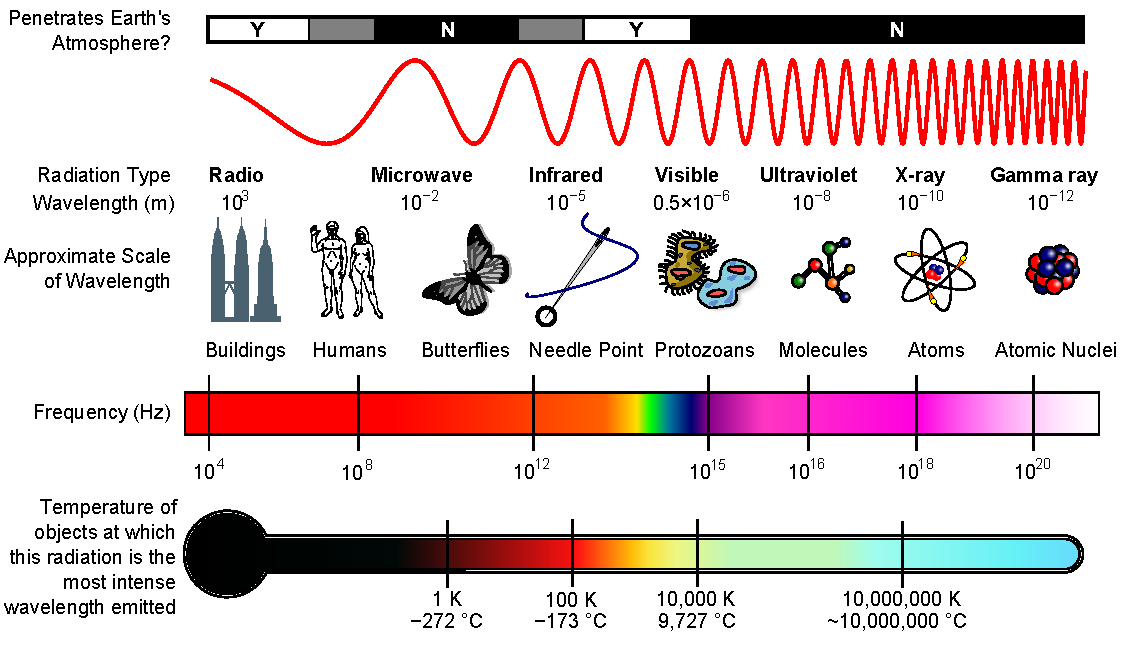
\includegraphics[width=1\linewidth]{fyz_fig006.pdf}
      \caption{Elektromagnetické spektrum (někdy zvané Maxwellova duha) zahrnuje elektromagnetické 
               záření všech možných vlnových délek. Srovnání délek elektromagnetických vln s 
               běžnými předměty a odpovídající teplotní stupnice umožňuje lépe získat představu o 
               jejich rozměrech a energiích.}
      \label{fyz:fig006}
    \end{figure}
    
    Elektromagnetické pole může přenášet vlny. Některé z těchto vln jsou světlo jak je znázorněno 
    na obrázku \ref{fyz:fig006}, jiné se používají při rádiovém vysílání, ale obecně se 
    nazývají \emph{elektromagnetickými vlnami}. Tyto vlny mohou mít rozmanité \emph{frekvence}. 
    Jediné, čím se jedna vlna liší od druhé, je právě frekvence vlnění. Kdybychom pohybovali 
    nábojem sem a tam a dělali bychom to stále rychleji a rychleji, objevovala by se celá řada 
    různých jevů, které je možné systematizovat udáním čísla vyjadřujícího počet kmitů za sekundu. 
    Frekvence, s nimiž přicházíme do styku prostřednictvím běžných rozvodových elektrických sítí v 
    domech, jsou řádově sto kmitů za sekundu. Zvýšíme-li frekvenci na \SI{500}{\kHz} nebo 
    \SI{1000}{\kHz} (\SI{1}{\kHz} = 1000 kmitů za sekundu), dostáváme se z domů ven, „na 
    vzduch“, neboť máme co činit s frekvencemi používanými při rozhlasovém vysílání. (Se vzduchem 
    to ale nemá co dělat! Rádiové vlny se mohou šířit i v prostoru, v němž není vzduch.) 
    Zvyšujeme-li frekvenci, dostáváme se do oblasti \emph{VKV} a televizního vysílání. Při ještě 
    vyšších frekvencích máme velmi krátké vlny, které se využívají např. v \emph{radiolokaci}. 
    Kdybychom šli ještě výše, nepotřebovali bychom už zařízení na registraci takových vln, protože 
    bychom je viděli naším zrakem. Kdybychom dokázali pohybovat nabitým hřebenem tak rychle, aby 
    kmital s frekvencemi od \SI{5e14}{\Hz} do \SI{5e15}{\Hz}, viděli bychom toto kmitání jako 
    červené, modré nebo fialové světlo v závislosti na frekvenci. Frekvence pod touto oblastí 
    nazýváme \emph{infračervenými} a nad touto oblastí \emph{ultrafialovými}. Skutečnost, 
    že naše vidění je omezeno na určitou frekvenční oblast, nedělá tuto oblast elektromagnetického 
    spektra z fyzikálního hlediska důležitější než jiné oblasti, avšak z lidského hlediska je tato 
    oblast přece jen zajímavější. Kdybychom frekvenci ještě zvýšili, dostali bychom 
    \emph{rentgenové paprsky}. Tyto paprsky nejsou nic jiného, než světlo s velmi vysokou 
    frekvencí. Ještě vyšším frekvencím odpovídá \emph{záření gama}. Výrazy rentgenové paprsky a 
    záření gama jsou téměř synonyma. Zářením gama nazýváme obvykle elektromagnetické vlny 
    pocházející z jader a rentgenovými paprsky vlny pocházející z atomů; při shodě jejich frekvencí 
    jsou však fyzikálně nerozlišitelné, bez zřetele na jejich původ. Vlny ještě vyšších 
    frekvencí, řekněme \SI{10e24}{\Hz}, lze získat uměle, například na \emph{synchrotronu} v 
    Caltechu. Elektromagnetické vlny úžasně vysokých frekvencí (až tisíckrát vyšších) je možné 
    najít ve vlnách \emph{kosmického záření}. Tyto vlny však neumíme ovládat. 
    \cite[s.~29]{Feynman02}
  
  \section{Kvantová Fyzika}\label{fyz:IchapIsecV}
    Když jsme načrtli představu elektromagnetického pole, v němž se mohou šířit vlny, brzy 
    zjistíme, že tyto vlny se chovají nezvykle, jako kdyby to ani vlny nebyly. Při vyšších 
    frekvencích se více podobají \emph{částicím}! Jejich neobvyklé chování vysvětluje 
    \emph{kvantová mechanika}, jejíž vznik je spojován s obdobím těsně po roce 1920. Před rokem 
    1920 pozměnil Einstein obraz trojrozměrného prostoru a nezávislého času nejdříve na kombinaci, 
    kterou nazýváme \emph{prostoročasem} a potom na \emph{zakřivený} prostoročas, aby vystihl 
    gravitaci. „Scéna“ se změnila na prostoročas a o gravitaci předpokládáme, že je modifikací 
    prostoročasu. Zjistilo se dokonce, že zákony pro pohyb částic jsou nepřesné. Mechanické zákony 
    „setrvačnosti“ a „síly“ jsou \emph{nesprávné} - Newtonovy zákony neplatí ve světě atomů. 
    Zjistilo se, že věci se v malém měřítku chovají úplně jinak než věci ve velkém měřítku. To dělá 
    fyziku obtížnou, ale velmi zajímavou. Obtížnou proto, že chování věcí malých rozměrů je pro nás 
    „nepřirozené“, nemáme v tomto směru přímé zkušenosti. Věci se tu chovají úplně jinak, než jsme 
    zvyklí, a proto není možné popsat jejich chování jinak, než analyticky. Takový popis je těžký a 
    vyžaduje mnoho představivosti.
    
    Kvantová mechanika má mnoho zvláštností. Především vylučuje předpoklad, že částice má určitou 
    polohu a určitou rychlost. Abychom ukázali, do jaké míry je klasická fyzika správná, uvedeme 
    pravidlo kvantové mechaniky, které říká, že není možné současně vědět, kde se něco nachází a 
    jak rychle se to pohybuje. Neurčitost v hybnosti a neurčitost v poloze jsou 
    \emph{komplementární} a jejich součin je konstantní. Můžeme to zapsat následujícím způsobem: 
    \(\Delta x \Delta p \frac{\si{\planckbar}}{2\pi}\). Podrobněji bude o tomto principu mluveno 
    později. Vysvětluje se tím velmi záhadný paradox: jsou-li atomy složeny z kladných a záporných 
    nábojů, proč se záporný náboj prostě neusadí na kladném náboji (tyto náboje se přitahují) a to 
    tak těsně, že by ho úplně vyrušil? \emph{Proč jsou atomy tak velké}? Proč je jádro uprostřed a 
    elektrony okolo něho? Zpočátku se myslelo, že příčinou je velký rozměr jádra; jenže jádro je 
    velmi malé. Atom má průměr okolo \SI{10e-10}{\meter}. Jádro má průměr asi \SI{10e-15}{\meter}. 
    Kdybychom měli atom a chtěli bychom vidět jeho jádro, museli bychom ho zvětšit tak, aby dosáhl 
    velikosti místnosti a i potom by bylo jádro malé jako skvrnka, kterou sotva spatříte okem, ale 
    téměř \emph{všechna hmotnost} atomu připadá na toto nepatrné jádro. Co brání elektronu prostě 
    spadnout na jádro? Právě uvedený princip. Kdyby elektrony byly v jádru, znali bychom přesně 
    jejich polohu a princip neurčitosti by si potom vyžadoval, aby měly velmi velkou (ale 
    \emph{neurčitou}) hybnost, tj. velmi velkou \emph{kinetickou energii}. S takovou energií by se 
    odtrhly od jádra. Dochází proto ke kompromisu: elektrony si ponechají jakýsi prostor pro tuto 
    neurčitost a potom se ve shodě s tímto pravidlem pohybují s jistým minimálním množstvím pohybu. 
    (Vzpomeňte si, že atomy krystalu při ochlazení na absolutní nulu neustaly ve svém pohybu, ale 
    přece jen kmitaly. Proč? Kdyby se přestaly pohybovat, věděli bychom, kde se nacházejí a že mají 
    nulový pohyb a to by bylo v rozporu s principem neurčitosti. Nemůžeme vědět, kde jsou a jak 
    rychle se pohybují; proto atomy musí neustále kmitat!)
    
    Jinou, velmi zajímavou změnou v ideách a filozofii vědy, kterou přinesla kvantová mechanika, je 
    nemožnost přesně předpovědět, co se za jakýchkoli daných okolností odehraje. Například, je 
    možné připravit atom, který bude emitovat světlo, a můžeme zjistit, kdy k této emisi došlo tím, 
    že zachytíme foton (o tomto si brzy řekneme více). Nemůžeme však dopředu předpovědět, kdy se 
    uskuteční emise světla, nebo v případě více atomů, který z nich bude emitovat světlo. Možná se 
    domníváte, že je to proto, že v atomu se nacházejí jakási vnitřní „kolečka“, která jsme ještě 
    nerozeznali. Ne, taková vnitřní kolečka neexistují! Příroda, tak jak ji dnes chápeme, se chová 
    tak, že je principiálně nemožné přesně předpovědět, co se skutečně stane v daném experimentu. 
    
    Opět se vrátíme ke kvantové mechanice a základní fyzice, ale nebudeme zabíhat do podrobností 
    kvantově mechanických principů, protože jsou dost těžké k pochopení. Budeme prostě předpokládat 
    jejich existenci a ukážeme, k jakým následkům vedou. Jedním z následků je, že věci, které jsme 
    považovali za vlny, se chovají jako částice a částice zase jako vlny; ve skutečnosti se tedy 
    všechno chová stejně. Není rozdíl mezi vlnou a částicí. \textbf{Kvantová mechanika sjednocuje 
    myšlenku pole, jeho vln a částic vjedno.} Při nízkých frekvencích je aspekt pole více zřejmý, 
    resp. užitečnější pro přibližný popis vyjádřený řečí naší každodenní zkušenosti. Se vzrůstem 
    frekvence však zařízení, které obvykle používáme v experimentu, poskytuje spíše důkazy o 
    částicích. I když mluvíme o vysokých frekvencích, musíme přiznat, že v oblasti frekvencí nad 
    \SI{10e12}{\Hz} nebyl zatím zjištěn žádný jev přímo související s frekvencí. K existenci 
    vyšších frekvencí docházíme pouze úvahou vycházející z energie částic a předpokladu správnosti 
    \emph{vlnově-korpuskulární představy kvantové mechaniky}.
    
    Takto docházíme i k novému pohledu na \emph{elektromagnetickou interakci}. Kromě elektronu, 
    protonu a neutronu existuje nový druh částice. Tuto částici nazýváme foton. Nový pohled na 
    interakci elektronů a protonů, tj. \emph{elektromagnetickou teorii}, která zároveň 
    \emph{splňuje} zákonitosti \emph{kvantové mechaniky}, nazýváme \emph{kvantovou 
    elektrodynamikou}. Tato základní teorie \emph{interakce světla a hmoty}, nebo 
    \emph{elektrického pole a nábojů}, je dosud největším úspěchem fyziky. V této jediné teorii 
    máme základní zákony, jimiž se řídí všechny známé jevy s výjimkou gravitace a jaderných 
    procesů. Pomocí kvantové elektrodynamiky můžeme vysvětlit všechny známé zákony mechaniky, 
    elektřiny a chemie. Plynou, zní zákony srážek kulečníkových koulí, pohyb vodičů v magnetickém 
    poli i tepelná kapacita oxidu uhelnatého, barva neonových reklam, hustota soli, reakce vodíku a 
    kyslíku při vzniku vody - to vše jsou následky jediného zákona. Všechny tyto detaily je možné 
    získat, je-li situace dost jednoduchá na to, abychom ji mohli přibližně popsat. To sice není 
    splněno téměř nikdy, často však můžeme pochopit více či méně, co se vlastně děje. Dosud se 
    neobjevily žádné výjimky ze zákonů kvantové elektrodynamiky, až na atomová jádra. O jádrech 
    však nemůžeme říci, jestli jde v jejich případě o výjimku, protože vlastně nevíme, jaké procesy 
    v nich probíhají. Při budování teorie jádra musíme překonat tři hlavní problémy:
    \begin{enumerate}
     \item Není znám přesný tvar sil působících mezi nukleony v jádře,
     \item rovnice popisující pohyb nukleonů v jádře jsou velmi komplikované – problém  
           matematického popisu,
     \item jádro má zároveň příliš mnoho nukleonů (nedá se popsat pohyb každé jeho částice) i    
           příliš málo (nedá se popsat jako makroskopické spojité prostředí).   
    \end{enumerate}
    Proto se musíme spokojit pouze s modely atomového jádra. 
    
    V podstatě je kvantová elektrodynamika teorií celé chemie a všech životních procesů, je-li 
    možné život v konečném důsledku redukovat na chemii, nebo vlastně na fyziku, protože chemie 
    vede k fyzice (a ta část fyziky, která se uplatňuje v chemii, je již dobře známá). Navíc, 
    kvantová elektrodynamika - ta úžasná vědní disciplína - předpověděla mnoho nových věcí. 
    Především mluví o vlastnostech fotonů velmi velkých energií, paprscích gama apod. Předpověděla 
    i jinou, velmi pozoruhodnou věc: kromě elektronu musí existovat jiná částice se stejnou 
    hmotností, ale s opačným nábojem, tzv. \emph{pozitron} a elektron s pozitronem mohou při srážce 
    anihilovat, přičemž se vyzáří světlo nebo paprsky gama (což je vlastně totéž, neboť světlo i 
    záření gama se liší polohou ve frekvenční škále elektromagnetických vln). Zobecnění poznatku, 
    že ke každé částici existuje antičástice, se ukazuje být pravdivým. V případě elektronů má 
    antičástice jiné jméno - nazývá se pozitronem, ale u většiny jiných částic mluvíme o anti-tom a 
    tom, např. o antiprotonu nebo antineutronu. Do kvantové elektrodynamiky se vkládají \emph{dvě 
    čísla} a o většině ostatních čísel ve světě se předpokládá, že jsou následkem těchto dvou. Tato 
    dvě vkládaná čísla nazýváme hmotností a nábojem elektronu. Ve skutečnosti to však není úplně 
    tak, neboť máme celý soubor chemických čísel, která hovoří o tom, jak těžká jsou jádra. To nás 
    přivádí k další kapitole.
  
  \section{Jádra a Částice}\label{fyz:IchapIsecVI}
    \emph{Z čeho jsou jádra a jak drží pohromadě}? Zjistilo se, že jádra jsou udržována obrovskými 
    silami. Při uvolnění těchto sil se uvolňuje energie, která je obrovská v porovnání s chemickou 
    energií, tak jak je obrovský výbuch atomové bomby v porovnání s výbuchem trinitrotoluenu. U 
    atomové bomby jde totiž o změny uvnitř jádra, zatímco výbuch trinitrotoluenu souvisí se změnami 
    elektronového obalu atomů. Proto si klademe otázku: co jsou to za síly, které udržují protony a 
    neutrony v jádře pohromadě? Tak, jako je možné elektrické působení přisoudit částici - fotonu, 
    předpokládal Yukawa, že i síly mezi neutrony a protony mají svá pole a kmity tohoto pole se 
    chovají jako částice. Kromě neutronů a protonů by proto měly existovat jiné částice a Yukawa 
    odvodil vlastnosti těchto částic z již známých charakteristik jaderných sil. Například, 
    předpověděl, že by měly mít hmotnost dvěstě až třistakrát větší než elektron; a div se 
    světe - v kosmickém záření byly objeveny částice s takovouto hmotností! Později se ukázalo, že 
    to nebyla ta správná částice. Tuto částici nazvali \(\mu\text{-mezon}\) neboli \emph{mion}.
    
    Trochu později, v roce 1947 nebo 1948, byla objevena jiná částice, \(\pi\text{-mezon}\) neboli 
    \emph{pion}, která vyhovovala Yukawovu kritériu. Abychom získali jaderné síly, musíme k protonu 
    a neutronu přidat pion. A teď si řeknete: „Och, jak velkolepé! - pomocí této teorie vybudujeme 
    nukleodynamiku, ve které budou mít piony takovou úlohu, jakou jim přisoudil Yukawa a všechno 
    bude vysvětleno“. Ta věc má však háček! Ukázalo se, že výpočty v této teorii jsou tak složité, 
    že se dodnes nikomu nepodařilo odvodit všechny důsledky této teorie, nebo ji porovnat s 
    experimentem; a to se už táhne spoustu let!
    
    Máme tedy teorii, ale nevíme, jestli je správná nebo nesprávná. Víme však už, že je trochu 
    chybná, nebo aspoň neúplná. Zatím co jsme marnili čas teorií a snažili se odvodit její 
    důsledky, experimentátoři některé věci objevili. Například, objevili \(\mu\text{-mezon}\) 
    neboli mion a my ani nevíme, jaká je jeho úloha. V kosmickém záření se našel velký počet 
    dalších „přebytečných“ částic. Dnes máme přibližně třista takových částic a je velmi těžké 
    porozumět vztahům mezi těmito částicemi a pochopit, na co je příroda potřebuje, nebo která z 
    nich na které závisí. Dnes tyto různé částice nechápeme jako různé aspekty téže věci a 
    skutečnost, že máme tak mnoho nesouvisejících částic, je odrazem toho, že máme tak mnoho 
    nesouvisejících informací bez dobré teorie. Po ohromném úspěchu kvantové elektrodynamiky máme 
    jisté znalosti z jaderné fyziky, ale jen hrubé znalosti, částečně experimentální a částečně 
    teoretické. Vycházíme přitom z charakteru sil působících mezi protony a neutrony a sledujeme, 
    co z toho vyplyne, ale v podstatě nechápeme, odkud ty síly pocházejí. Kromě toho nebylo 
    dosaženo téměř žádného pokroku. Objevili jsme velký počet chemických prvků. Mezi těmito prvky 
    se najednou objevila souvislost, neočekávaná souvislost zakotvená v Mendělejevově periodické 
    tabulce prvků. Například, sodík a draslík jsou téměř shodné ve svých chemických vlastnostech a 
    v Mendělejevově tabulce se nacházejí ve stejném sloupci. Hledala se tabulka Mendělejevova typu 
    pro nové částice. Taková tabulka nových částic byla sestavena nezávisle Gell-Mannem v USA a 
    Nishijimou v Japonsku. Základem jejich klasifikace je nové číslo, jež je možno, podobně jako 
    elektrický náboj, přiřadit každé částici a které se nazývá její „podivností“ S (od anglického 
    slova strangeness). Toto číslo se, podobně jako elektrický náboj, zachovává v reakcích 
    vyvolávaných jadernými silami.  
   
%} %tikzset
%~~~~~~~~~~~~~~~~~~~~~~~~~~~~~~~~~~~~~~~~~~~~~~~~~~~~~~~~~~~~~~~~~~~~~~~~~~~~~~~~~~~~~~~~~~~~~~~~~~
\printbibliography[title={Seznam literatury}, heading=subbibliography]
\addcontentsline{toc}{section}{Seznam literatury}
